\documentclass[12pt]{report}

% Metadata
\title{Applicare il Machine Learning per il Rilevamento dello Stress negli Ambienti di Lavoro di Ufficio}
\author{Roberto Vicario}

% Language and Encoding Settings
\usepackage[italian]{babel}

% Formatting and Layout
\usepackage{geometry}
\geometry{
    top=3cm,
    left=2.5cm,
    right=2.5cm,
    bottom=3cm
}
\setlength{\parindent}{0pt}
\usepackage{fancyhdr}
\usepackage{setspace}
\usepackage{float}
\usepackage{multicol}

% Fonts and Typography
\usepackage{fontspec}
\setmainfont{Arial}
\usepackage{lipsum}
\usepackage{xcolor}

% Graphics
\usepackage{graphicx}
\usepackage{svg}

% Mathematics and programming
\usepackage{amsmath}
\usepackage{amssymb}
\usepackage{listings}
\lstset{
    language=Python,
    frame=tlrb,
    aboveskip=3mm,
    belowskip=6mm,
    showstringspaces=false,
    columns=flexible,
    basicstyle={\small\ttfamily},
    numbers=left,
    numberstyle=\tiny\color{black}\ttfamily,
    numbersep=4pt,
    keywordstyle=\color{black},
    commentstyle=\color{black},
    stringstyle=\color{black},
    breaklines=true,
    breakatwhitespace=true,
    tabsize=2
}

% Hyperlinks
\usepackage[
    colorlinks=true,
    linkcolor=black,
    citecolor=black,
    urlcolor=black,
]{hyperref}

% Bibliography and References
\usepackage{biblatex}
\addbibresource{pages/references.bib}

\begin{document}

\pagestyle{empty}

\begin{center}
    \includesvg[width=0.25\linewidth]{img//UNINSUBRIA-Logo.svg}
    
    \vspace*{\fill}
    
    \Large

    Università degli Studi dell'Insubria
    
    Dipartimento di Scienze Teoriche e Applicate (DiSTA)

    Corso di Laurea triennale in Informatica
    
    \vspace*{\fill}
    
    \LARGE
    
    \textbf{Applicare il Machine Learning per il Rilevamento dello Stress negli Ambienti di Lavoro di Ufficio}
    
    \vspace*{\fill}
    
    \Large
    
    \begin{multicols}{2}
        \begin{flushleft}
            Relatrice: \\
            Dott.ssa Silvia Corchs
        \end{flushleft}
        
        \columnbreak
    
        \begin{flushright}
            Candidato: \\
            Roberto Vicario \\
            Matricola 744072
        \end{flushright}
    \end{multicols}
    
    \vspace*{\fill}
    
    Anno Accademico: 2022/2023
\end{center}
\newpage
\thispagestyle{empty}
\mbox{}
\pagebreak

\pagestyle{fancy}

\fancyhf{}

\fancyhead[C]{Ringraziamenti}
\fancyfoot[C]{}

\fancypagestyle{plain}{
    \fancyhf{}
    \fancyfoot[C]{}
}

\chapter*{Ringraziamenti}

\large

Innanzitutto, vorrei ringraziare la mia relatrice, la Dott.ssa Silvia Corchs. Ho trovato la ricerca da lei suggerita particolarmente innovativa e appagante rispetto ad altre proposte; questo mi ha dato modo di mettermi in gioco nel lavoro e di sviluppare una passione per la data science. Le sono anche grato per i preziosi consigli forniti riguardo al mio percorso post Laurea e su come poter rendere più competitiva la mia figura professionale.

\bigskip

Vorrei ringraziare di cuore Cecilia, l'unica persona che ha saputo tirare fuori il meglio di me e farmi credere nelle mie potenzialità. La tua presenza nella mia vita è diventata un pilastro fondamentale, e non posso fare a meno di ricordare ciò che sei diventata per me: sei la mia compagna di vita, complice di avventure e sostenitrice in ogni momento.

\bigskip

Ringrazio mamma e papà; nonostante le difficoltà che abbiamo affrontato, mi avete dato tutto. Grazie a voi, oggi mi trovo qui a riflettere su ciò che ho, anziché concentrarmi su ciò che mi è mancato. Una dedica speciale va mia sorella Ilaria; auguro che tu possa scoprire le tue passioni e realizzare i tuoi sogni, proprio come è successo a me, trovando in essi la felicità e la pace.

\bigskip

Un pensiero speciale è dedicato a Chiara, che ci ha lasciato alcuni mesi fa. Ho sempre immaginato la tua presenza alla mia festa di Laurea; avrei comprato quei cannoli al pistacchio che ti piacevano tanto. Ci sono aspetti che avevo progettato e che credevo si sarebbero realizzati sicuramente, anche cose banali come questa, ma la vita è strana e non riesco a capire perché tu abbia dovuto affrontare questo destino. Voglio ricordarti e portarti con me anche per festeggiare questo traguardo.
\newpage
\thispagestyle{empty}
\mbox{}
\pagebreak

\setcounter{page}{1}
\pagenumbering{Roman}

\pagestyle{fancy}

\fancyhf{}

\fancyhead[C]{Indice}
\fancyfoot[C]{\thepage}

\fancypagestyle{plain}{
    \fancyhf{}
    \fancyfoot[C]{\thepage}
}

\large

\tableofcontents

\listoffigures

\listoftables
\newpage
\thispagestyle{empty}
\mbox{}
\pagebreak

\setcounter{page}{1}
\pagenumbering{arabic}

\setcounter{chapter}{0}
\pagestyle{fancy}

\fancyhf{}

\fancyhead[C]{Introduzione}
\fancyfoot[C]{\thepage}

\fancypagestyle{plain}{
    \fancyhf{}
    \fancyfoot[C]{\thepage}
}

\chapter{Introduzione}

\large

Il rilevamento dello stress negli ambienti di lavoro, rappresenta un elemento innovativo per promuovere la salute e il benessere dei dipendenti, soprattutto negli embienti di lavoro d'ufficio. L'utilizzo del machine learning in questo caso offre un approccio efficace per identificare segnali precoci di stress, consentendo alle organizzazioni di intervenire tempestivamente per mitigare i rischi associati. In particolare, è di nostro interesse esaminare se i risultati ottenuti attraverso metodi di apprendimento non supervisionato possano essere paragonabili a quelli derivanti da approcci supervisionati, come evidenziato nella ricerca \textit{"Exploring Unsupervised Machine Learning Classification Methods for Physiological Stress Detection"} di Iqbal et al. (2022) \cite{iqbal2022exploring}.

\bigskip

Il dataset SWELL-KW, è stata la risorsa fondamentale da cui prelevare i dati per allenare i modelli di intelligenza artificiale a intercettare lo stress nei lavoratori dipendenti. All'interno del capitolo, viene esplorato il processo di raccolta dei dati, delineando le metodologie utilizzate per garantire la qualità del dataset. Successivamente, vengono analizzate le features estratte dai dati e le relative labels associate.

\bigskip

In seguito, si procede con l'analisi dei segnali biomedici, attribuendo loro un'importanza fondamentale nel contesto della ricerca. Viene esposta la distinzione tra segnali fisici e fisiologici, con un focus approfondito sugli specifici segnali impiegati. Particolarmente rilevante è la frequenza cardiaca, rappresentata tramite l'elettrocardiogramma (ECG), che assume un ruolo fondamentale nelle indagini sul rilevamento dello stress. L'esplorazione di questi temi costituisce una base essenziale per comprendere le principali metodologie di machine learning nell'ambito della variabilità della frequenza cardiaca (HRV).

\bigskip

Successivamente, vengono presentate le ricerche allo stato dell'arte sul rilevamento dello stress utilizzando metodi di machine learning. Le metodologie e i risultati esposti nel capitolo quattro rivestono un'importanza cruciale nel tracciare lo stato attuale della ricerca e nel fornire un contesto significativo per future indagini. Questi elementi sono particolarmente rilevanti per la definizione delle metodologie e la comparazione dei risultati ottenuti in questo progetto.

\bigskip

Infine, si espone la metodologia adottata, a partire dalle tecnologie impiegate nello sviluppo del progetto fino ai metodi di machine learning utilizzati per apprendere e valutare i risultati. Nei capitoli cinque e sei, il progetto è dettagliato sia dal punto di vista teorico che pratico, approfondendo l'analisi che ha condotto all'implementazione. In conclusione, vengono presentati e confrontati i risultati ottenuti dai modelli generati tramite queste metodologie con quelli allo stato dell'arte. Infine, si delineano le linee guida per future ricerche sul rilevamento dello stress mediante l'utilizzo del machine learning, sfruttando il dataset SWELL-KW per analizzare lo stress negli ambienti di lavoro d'ufficio.
\pagebreak

\setcounter{chapter}{1}
\pagestyle{fancy}

\fancyhf{}

\fancyhead[C]{Dataset SWELL-KW}
\fancyfoot[C]{\thepage}

\fancypagestyle{plain}{
    \fancyhf{}
    \fancyfoot[C]{\thepage}
}

\chapter{Dataset SWELL-KW}

\large

IL dataset SWELL-KW (SWELL Knowledge Work) è un insieme di dati multimodali raccolti in un esperimento, documentato in \textit{"The swell knowledge work dataset for stress and user modeling research"} di Koldijk et al. (2014) \cite{koldijk2014swell}. L'esperimento ha coinvolto 25 partecipanti che svolgevano compiti tipici del knowledge work. Il dataset include dati sui modelli di digitazione, sui movimenti del mouse, sulla pressione dei tasti e sul comportamento dello sguardo dei partecipanti, nonché sulla loro esperienza soggettiva di carico del compito, sforzo mentale, emozione e stress percepito.

\bigskip

Questo dataset è utile, in particolare utilizzando i segnali fisiologici, per sviluppare modelli di machine learning per classificare lo stress sul posto di lavoro. Questi modelli possono poi essere utilizzati per fornire un feedback in tempo reale agli utenti o per regolare l'interfaccia utente in modo che sia di maggior supporto.

\bigskip

Il dataset SWELL-KW è una risorsa preziosa per il rilevamento dello stress. Tuttavia, è importante notare che il dataset presenta alcune limitazioni:

\begin{itemize}
    \item I dati raccolti si basano sull'esperienza di soli 25 partecipanti. Questo limita la generalizzabilità dei risultati a una popolazione più ampia.
    \item I compiti sono stati organizzati su attività di lavoro conosciute dagli individui. Questa situazione potrebbe non rendere la ricerca applicabile ad altre tipologie di impieghi, come lavori creativi, che richiedono più inventiva che metodologia.
\end{itemize}

\section{Raccolta dei dati}

\begin{table}[t]
    \centering
    \begin{tabular}{|ll|}
        \hline
        \textbf{Tipo}
        & \textbf{Features} \\
        \hline
        Interazioni con il computer
        & Mouse (3) \\ 
        & Tastiera (7) \\
        & Applicazioni (2) \\
        Espressioni facciali
        & Orientamento della testa (3) \\
        & Movimenti del viso (10) \\
        & Unità di azione (19) \\
        & Emozione (8) \\
        Posture del corpo
        & Distanza (1) \\
        & Angoli di giunzione (10) \\
        & Orientamenti delle ossa (3 x 11) \\
        Fisiologia
        & HRV (2) \\
        & Conduttanza cutanea (1) \\
        \hline
    \end{tabular}
    \caption{Features raccolte durante l'esperimento.}
    \label{tab:2-1}
\end{table}

Durante l'esperimento, i partecipanti hanno svolto una serie di compiti conosciuti, come scrivere relazioni, fare presentazioni, leggere e-mail e cercare informazioni. Durante ogni compito, ai partecipanti è stato anche chiesto di eseguire un compito stressante. La raccolta dei dati è stata condotta utilizzando una serie di sensori, tra cui una webcam, un sensore della tastiera, un sensore del mouse e un eye tracker. I sensori sono stati utilizzati per raccogliere dati sui modelli di digitazione dei partecipanti, sui movimenti del mouse, sulla pressione dei tasti e sul comportamento dello sguardo.

\bigskip

Oltre ai dati dei sensori, i partecipanti hanno completato una serie di questionari per valutare la loro esperienza soggettiva del carico di lavoro, dello sforzo mentale, delle emozioni e dello stress percepito. Questi questionari hanno fornito una verità di base per i dati del sensore, consentendo ai ricercatori di collegare il comportamento osservato alle esperienze soggettive dei partecipanti.

\bigskip

In conclusione, dopo una sintesi dei dati raccolti, è possibile osservare una rappresentazione completa e organizzata delle features ricavate nella tabella \ref{tab:2-1}.

\section{Analisi delle features}

\begin{table}[t]
    \centering
    \begin{tabular}{|lp{0.5\linewidth}|}
        \hline
        \textbf{Feature}
        & \textbf{Descrizione} \\
        \hline
        MEAN\_RR
        & Media di tutti gli intervalli RR. \\
        MEDIAN\_RR
        & Mediana di tutti gli intervalli RR \\
        SDRR
        & Deviazione standard di tutti gli intervalli RR. \\
        RMSSD
        & Radice quadrata della media della somma dei quadrati della differenza tra gli intervalli RR adiacenti. \\
        SDSD
        & Deviazione standard delle differenze tra intervalli RR adiacenti. \\
        SDRR\_RMSSD
        & Rapporto tra SDRR e RMSSD. \\
        HR
        & Frequenza cardiaca. \\
        pNN25
        & Percentuale di intervalli RR adiacenti che differiscono di oltre 25 ms. \\
        pNN50
        & Percentuale di intervalli RR adiacenti che differiscono di oltre 50 ms. \\
        SD1
        & Descrittore del grafico di Poincaré dell'HRV a breve termine. \\
        SD2
        & Descrittore del grafico di Poincaré dell'HRV a lungo termine. \\
        KURT
        & Curtosi di tutti gli intervalli RR. \\
        SKEW
        & Skewness di tutti gli intervalli RR. \\
        \hline
    \end{tabular}
    \caption{Features fondamentali nel dataset SWELL-KW.}
    \label{tab:2-2}
\end{table}

Lo studio \textit{"Thermal Comfort and Stress Recognition in Office Environment"} di Nkurikiyeyezu et al. (2014) \cite{nkurikiyeyezu2019thermal} fornisce una visione d'insieme delle features estratte dal dataset SWELL-KW. Nella tabella \ref{tab:2-2}, sono illustrate e descritte le features estratte che sono state scelte e impiegate nel progetto presentato in questa tesi. Le seguenti features possono essere considerate fondamentali, poiché derivano da operazioni statistiche elementari, come la media, la mediana e altre, applicate ai segnali fisiologici campionati.

\subsection{Frequenza relativa degli intervalli RR}

\begin{table}[t]
    \centering
    \begin{tabular}{|lp{0.5\linewidth}|}
        \hline
        \textbf{Feature}
        & \textbf{Descrizione} \\
        \hline
        MEAN\_REL\_RR
        & Media di tutti gli intervalli RR relativi. \\
        MEDIAN\_REL\_RR
        & Mediana di tutti gli intervalli RR relativi. \\
        SDRR\_REL\_RR
        & Deviazione standard di tutti gli intervalli RR relativi. \\
        RMSSD\_REL\_RR
        & Radice quadrata della media della somma dei quadrati della differenza tra intervalli RR relativi adiacenti. \\
        SDSD\_REL\_RR
        & Deviazione standard di tutti gli intervalli di differenze tra intervalli RR relativi adiacenti. \\
        SDRR\_RMSSD\_REL
        & Rapporto tra SDRR\_REL e RMSSD\_REL. \\
        KURT\_REL\_RR
        & Curtosi di tutti gli intervalli RR relativi. \\
        SKEW\_REL\_RR
        & Skewness di tutti gli intervalli RR relativi. \\
        \hline
    \end{tabular}
    \caption{Features del dataset SWELL-KW basate sulla frequenza relativa degli intervalli RR.}
    \label{tab:2-3}
\end{table}

All'interno del dataset sono disponibili altre features, come è possibile osservare dalla tabella \ref{tab:2-3}. Queste features hanno il nome di quelle precedentemente presentate nella tabella \ref{tab:2-2}, con l'aggiunta della dicitura "\_REL\_RR", che indica "frequenza relativa agli intervalli RR". Per comprenderne il significato, è necessario fare riferimento alle nozioni statistiche di frequenza assoluta e frequenza relativa. La frequenza assoluta rappresenta il conteggio dei casi in una feature specifica. La frequenza relativa, invece, offre una prospettiva in percentuale su quanto una feature sia rappresentata rispetto all'intervallo RR. Le features presenti nella tabella \ref{tab:2-2} sono basate su frequenza assoluta, mentre quelle presenti nella tabella \ref{tab:2-3} utilizzano la frequenza relativa, entrambe le categorie su intervalli RR.

\bigskip

Per un'analisi più dettagliata sull'argomento, è stato preso in considerazione lo studio \textit{"A robust, simple and reliable measure of heart rate variability using relative RR interval"} di Vollmer et al. (2015) \cite{vollmer2015robust}.

\subsection{Potenza di campionamento del segnale}

\begin{table}[t]
    \centering
    \begin{tabular}{|lp{0.5\linewidth}|}
        \hline
        \textbf{Feature}
        & \textbf{Descrizione} \\
        \hline
        VLF
        & Banda di frequenza molto bassa dello spettro di potenza dell'HRV. \\
        LF
        & Banda di frequenza bassa dello spettro di potenza dell'HRV. \\
        HF
        & Banda di frequenza alta dello spettro di potenza dell'HRV. \\
        TP
        & Spettro di potenza totale HRV. \\
        LF/HF
        & Rapporto tra LF e HF. \\
        HF/LF
        & Rapporto tra HF e LF. \\
        sampen
        & Entropia del campione del segnale RR. \\
        higuci
        & Dimensione frattale di Higuchi. \\
        \hline
    \end{tabular}
    \caption{Features del dataset SWELL-KW basate sulla potenza di campionamento del segnale.}
    \label{tab:2-5}
\end{table}

La tabella \ref{tab:2-5}, presenta l'ultimo insieme di features, le quali condividono tutte l'attributo comune di essere basate sulla potenza di campionamento, focalizzandosi specificamente sulla banda di frequenza dello spettro di potenza.

\bigskip

Per ottenere una comprensione più dettagliata di queste features, è stato fatto riferimento principalmente allo studio \textit{"A robust, simple and reliable measure of heart rate variability using relative RR interval"} di Vollmer et al. (2015) \cite{vollmer2015robust}. Per la feature sampen, è stata consultata la ricerca \textit{"Advances in heart rate variability signal analysis: joint position statement by the e-Cardiology ESC Working Group and the European Heart Rhythm Association co-endorsed by the Asia Pacific Heart Rhythm Society"} di Sassi et al. (2015) \cite{sassi2015advances}. Per la feature higuci, è stato consultato lo studio \textit{"Higuchi fractal analysis of heart rate variability is sensitive during recovery from exercise in physically active men"} di Gomes et al. (2017) \cite{gomes2017higuchi}.

\section{Analisi delle labels}

Come illustrato precedentemente, i partecipanti coinvolti nell'esperimento sono stati soggetti a circostanze particolari durante lo svolgimento delle attività lavorative. Questo approccio mirava a categorizzare e valutare il livello di stress, in tre situazioni:

\begin{itemize}
    \item \textbf{No stress}: In questa condizione, i partecipanti hanno avuto la libertà di lavorare secondo i propri ritmi senza pressioni esterne. Dopo 45 minuti dall'inizio dell'attività, è stato loro chiesto di fermarsi. Questo scenario è stato considerato come un riferimento per uno stato di nessun stress.
    \item \textbf{Time pressure}: Per simulare uno stress moderato, ai partecipanti è stato dato un tempo limitato di 30 minuti per completare le loro attività. Questa condizione rappresenta una situazione di pressione temporale che si può riscontrare frequentemente nell'ambiente lavorativo.
    \item \textbf{Interruption}: Questa condizione è stata considerata come il livello massimo di stress. Non sono stati forniti dettagli specifici su come è stata implementata questa interruzione, ma si intuisce che si tratti di un evento o una serie di eventi che hanno portato i partecipanti a vivere una situazione di forte disagio o interruzione del flusso di lavoro.
\end{itemize}

\section{Informazioni sul dataset}

Il dataset SWELL-KW è accessibile pubblicamente per il download tramite la piattaforma \href{https://www.kaggle.com/datasets/qiriro/swell-heart-rate-variability-hrv}{\underline{Kaggle}}. All'interno di questa risorsa, è possibile reperire il dataset elaborato in file CSV, opportunamente diviso in train e testing set. La distribuzione di tali insiemi è stata configurata con una proporzione del 70\% per l'addestramento e del 30\% per il test. Complessivamente, il dataset comprende oltre 400.000 tuple, fornendo un ampio spettro di dati per le analisi e le applicazioni desiderate.
\pagebreak

\setcounter{chapter}{2}
\pagestyle{fancy}

\fancyhf{}

\fancyhead[C]{Segnali biomedici}
\fancyfoot[C]{\thepage}

\fancypagestyle{plain}{
    \fancyhf{}
    \fancyfoot[C]{\thepage}
}

\chapter{Segnali biomedici}

\begin{figure}[t]
    \centering
    \includegraphics[width=\linewidth]{img//3/1.png}
    \caption{Principali segnali utilizzati nel rilevamento dello stress.}
    \label{fig:3-1}
\end{figure}

La figura \ref{fig:3-1}, tratta da \textit{"Review on psychological stress detection using biosignals"} di Giannakakis et al. (2019) \cite{giannakakis2019review}, illustra i principali segnali utilizzati nelle ricerche attinenti alla tematica della rilevazione dello stress.

\bigskip

In ricerche analoghe, sono stati utilizzati segnali sia fisici che fisiologici, in questa tesi, si è dato rilievo esclusivamente ai segnali fisiologici.

\bigskip

La categoria dei segnali fisici comprende misure direttamente correlate a grandezze fisiche. La raccolta di tali segnali avviene mediante l'utilizzo di sensori e strumentazione fisica specializzata. Questi segnali forniscono informazioni concrete e tangibili, spesso sotto forma di dati numerici, che possono essere analizzati per ottenere una valutazione accurata delle condizioni fisiche dell'organismo.

\bigskip

I segnali fisiologici comprendono misure che riflettono il normale funzionamento dei processi fisiologici all'interno dell'organismo. Questi segnali offrono una finestra sulle attività biologiche e metaboliche del corpo, consentendo agli operatori sanitari e ai ricercatori di comprendere meglio il funzionamento interno dell'organismo.

\section{Frequenza cardiaca}

La frequenza cardiaca è un parametro fisiologico, e si riferisce al numero di battiti cardiaci per unità di tempo, solitamente misurati in battiti al minuto. Questo parametro può essere descritto utilizzando l'equazione \ref{eq:3-1}.

\begin{equation}
    \boxed{
    \text{HR} = \frac{\text{Heart beats}}{\text{Minutes}}
    }
    \label{eq:3-1}
\end{equation}

\bigskip

Per un adulto, la frequenza cardiaca a riposo varia in genere da 60 a 100 battiti al minuto. Tuttavia, fattori come l'età, il livello di forma fisica e la salute generale possono influenzare la frequenza cardiaca di base di un individuo.

\subsection{Elettrocardiografia}

L'elettrocardiografia (ECG) è un processo che registra l'attività elettrica del cuore in un intervallo di tempo specifico. L'attività elettrica del cuore genera piccole correnti elettriche, l'elettrocardiografia cattura questi segnali elettrici e produce una rappresentazione grafica dell'attività cardiaca. Gli elettrodi, sotto forma di cerotti adesivi, vengono posizionati sulla pelle per catturare i segnali elettrici da diverse aree del cuore. I posizionamenti standard includono gli arti e il torace.

\subsection{Elettrocardiogramma}

\begin{figure}[t]
    \centering
    \includegraphics[width=\linewidth]{img//3/2.png}
    \caption{Esempio di elettrocardiogramma (ECG) che mostra gli impulsi elettrici generati dal cuore durante ogni ciclo cardiaco.}
    \label{fig:3-2}
\end{figure}

L'elettrocardiogramma è una rappresentazione grafica, nonché l'output, prodotto dal processo di elettrocardiografia. L'elettrocardiogramma è quindi un grafico che mostra gli impulsi elettrici generati dal cuore durante ogni ciclo cardiaco.

\bigskip

La figura \ref{fig:3-2}, tratta dallo studio \textit{"A survey on ECG analysis"} di Berkaya et al. (2018) \cite{berkaya2018survey}, mostra un esempio di elettrocardiogramma. L'immagine raffigurata include diverse nomenclature; saranno prese in considerazione solo quelle che si sono rivelate utili per sviluppare la ricerca:

\begin{enumerate}
    \item \textbf{Onda P}: Rappresenta l'attività atriale, indicando la depolarizzazione degli atrii.
    \item \textbf{Complesso QRS}: Indica la depolarizzazione dei ventricoli. È composto da onde Q, R e S.
    \item \textbf{Onda T}: Rappresenta la ripolarizzazione dei ventricoli.
\end{enumerate}

\subsection{Intervallo RR}

L'intervallo RR è il tempo, rappresentato in millisecondi, che intercorre tra le onde R consecutive in un elettrocardiogramma. Questo intervallo è fondamentale poiché riflette il tempo tra due depolarizzazioni ventricolari consecutive. La periodicità di questo intervallo, che rende misurabile la frequenza cardiaca, può essere analizzata ulteriormente attraverso la trasformata di Fourier, evidenziando così le componenti frequenziali del segnale cardiaco. Un intervallo RR può essere rappresentato come illustrato nell'equazione \ref{eq:3-2}.

\begin{equation}
    \boxed{
    \text{RR interval} = \text{R}_{i+1}(t) - \text{R}_i(t)
    }
    \label{eq:3-2}
\end{equation}

\bigskip

Dove, $R_i(t)$ rappresenta il tempo di occorrenza del $i$-esimo picco R e $R_{i+1}(t)$ il tempo del successivo picco R.

\subsection{Heart Rate Variability}

L'intervallo RR costituisce un elemento cruciale per la valutazione della HRV (Heart Rate Variability), parametro che è da lungo tempo un elemento cardine nello stato dell'arte per studi che riguardano la classificazione dello stress.

\bigskip

A titolo esemplificativo, si menziona il lavoro intitolato \textit{"Comparison of heart rate variability measures for mental stress detection"} di Boonnithi et al. (2011) \cite{boonnithi2011comparison}. In questo studio, gli autori hanno confrontato diverse misure della HRV per determinare la loro efficacia nel rilevare lo stress mentale.
\pagebreak

\setcounter{chapter}{3}
\pagestyle{fancy}

\fancyhf{}

\fancyhead[C]{Stato dell'arte}
\fancyfoot[C]{\thepage}

\fancypagestyle{plain}{
    \fancyhf{}
    \fancyfoot[C]{\thepage}
}

\chapter{Stato dell'arte}

\large

In questo capitolo, vengono illustrate le attuali ricerche di rilievo nello stato dell'arte relative al rilevamento dello stress mediante l'impiego di metodologie di machine learning.

\section{Real-time stress detection}

\begin{figure}[t]
    \centering
    \includegraphics[width=\linewidth]{img//4/1.png}
    \caption{Implementazione pratica di un sistema di monitoraggio dello stress.}
    \label{fig:4-1}
\end{figure}

Lo studio \textit{"Stress Monitoring Using Machine Learning, IoT, and Wearable Sensors"} di Al-Atawi et al. (2023) \cite{al2023stress} esplora l'integrazione di machine learning, internet of things (IoT) e sensori indossabili, i cosidetti "wearables", per il monitoraggio dello stress in tempo reale.

\bigskip

In un'implementazione pratica, come illustrato dalla figura \ref{fig:2-1}, tratta dallo studio di Khowaja et al. (2021) \cite{khowaja2021toward}, un sistema di monitoraggio dello stress, si sviluppa in queste fasi operative:

\paragraph{Raccolta dei dati}

I dati possono essere raccolti da wearables, come smartwatch, braccialetti fitness o occhiali intelligenti. Questi sensori possono misurare una varietà di parametri fisiologici, tra cui la frequenza cardiaca, la respirazione, la temperatura della pelle e l'attività muscolare.

\paragraph{Classificazione e previsione dei risultati}

La fase di classificazione e previsione dei risultati è quella in cui i dati raccolti vengono elaborati per identificare i livelli di stress. I metodi di classificazione e previsione possono essere basati su machine learning.

\paragraph{Presentazione dei risultati}

I risultati possono essere utilizzati per identificare le persone che sono a rischio di stress o che hanno già livelli di stress elevati. Queste informazioni vengono quindi trasmesse agli utenti finali attraverso applicativi dedicati.

\section{Stress detection con modelli non supervisionati}

Lo studio \textit{"Exploring Unsupervised Machine Learning Classification Methods for Physiological Stress Detection"} di Iqbal et al. (2022) \cite{iqbal2022exploring} analizza l'efficacia dei metodi non supervisionati per il rilevamento dello stress utilizzando segnali fisiologici. Gli autori valutano diversi metodi, tra cui affinity propagation e mean shift, estraendo le features dal dataset SWELL-KW.

\bigskip

I risultati dimostrano che i metodi di machine learning non supervisionati ottengono prestazioni paragonabili o superiori ai metodi supervisionati tradizionali su entrambi dataset. Affinity propagation e mean shift hanno mostrato le migliori performance, con punteggi F1 dell'80.10\% e del 78.05\%, rispettivamente. Anche k-means e mini-batch k-means hanno ottenuto buoni risultati, con punteggi F1 del 74.10\% e del 71.70\%, rispettivamente.

\section{Stress detection con modelli non supervisionati di rilevamento delle anomalie}

Lo studio \textit{"Evaluating different configurations of machine learning models and their transfer learning capabilities for stress detection using heart rate"} di Albaladejo-González et al. (2023) \cite{albaladejo2023evaluating} studia l'efficacia di vari modelli di apprendimento automatico nel rilevare lo stress sulla base dei dati della frequenza cardiaca. Gli autori analizzano diversi modelli supervisionati, incluso Multi-layer Perceptron (MLP), e altri modelli non supervisionati di rilevamento delle anomalie, tra cui Local Outlier Factor (LOF), estraendo le features dal dataset SWELL-KW.

\bigskip

Gli autori hanno valutato le prestazioni di ciascun modello utilizzando il punteggio F1, una metrica che considera sia la precisione che il richiamo. I risultati hanno mostrato che i modelli di rilevamento delle anomalie non supervisionati hanno superato i modelli supervisionati su entrambi i dataset. LOF ha ottenuto i punteggi F1 più elevati, pari al 77.17\%. Anche MLP ha ottenuto buoni risultati, con un punteggio F1 dell'82.75\%.

\section{Stress detection con modelli di deep learning}

Lo studio \textit{"Multi-Class Stress Detection through Heart Rate Variability: A Deep Neural Network based Study"} di Mortensen et al. (2023) \cite{mortensen2023multi} presenta un approccio innovativo al rilevamento dello stress, impiegando Deep Neural Network (DNN) per la classificazione ed estraendo le features dal dataset SWELL-KW.

\bigskip

I risultati dimostrano che il DNN proposto ha raggiunto un'elevata precisione, con un punteggio F1 del 99.80\% sui tre livelli di stress. Gli autori attribuiscono questo successo alla capacità delle DNN di apprendere modelli e relazioni complesse nei dati HRV.

\section{Risultati dei modelli}

\begin{table}[t]
    \centering
    \begin{tabular}{|lll|}
        \hline
        \textbf{Studio}
        & \textbf{Modello}
        & \textbf{Punteggio} \\
        \hline
        \cite{iqbal2022exploring}
        & Affinity propagation
        & 80.10\% \\
        \cite{iqbal2022exploring}
        & Mean shift
        & 78.05\% \\
        \cite{albaladejo2023evaluating}
        & Local Outlier Factor (LOF)
        & 77.17\% \\
        \cite{albaladejo2023evaluating}
        & Multi-layer Percepton (MLP)
        & 82.75\% \\
        \cite{mortensen2023multi}
        & Deep Neural Network (DNN)
        & 99.80\% \\
        \hline
    \end{tabular}
    \caption{Risultati dei modelli allo stato dell'arte.}
    \label{tab:4-1}
\end{table}

La tabella \ref{tab:4-1} offre un panorama completo dei risultati ottenuti nelle ricerche precedenti. Risalta in modo evidente l'eccezionale successo dei modelli di deep learning, i quali ottengono risultati straordinariamente elevati per questo tipo di ricerche. Al contrario, i metodi non supervisionati si distinguono per la loro robustezza, sebbene i loro risultati siano inferiori in confronto.
\pagebreak

\setcounter{chapter}{4}
\pagestyle{fancy}

\fancyhf{}

\fancyhead[C]{Metodologia}
\fancyfoot[C]{\thepage}

\fancypagestyle{plain}{
    \fancyhf{}
    \fancyfoot[C]{\thepage}
}

\chapter{Metodologia}

\large

In questo capitolo, viene esposta la metodologia adottata, partendo dalle tecnologie impiegate nello sviluppo del progetto fino ai metodi di machine learning utilizzati per apprendere e valutare i risultati.

\section{Sviluppo del progetto}

\begin{table}[t]
    \centering
    \begin{tabular}{|ll|}
        \hline
        \textbf{Libreria}
        & \textbf{Descrizione} \\
        \hline
        \texttt{numpy}
        & Utilizzata per calcoli numerici avanzati. \\
        \texttt{scipy}
        & Estende numpy per il calcolo scientifico più complesso. \\
        \texttt{pandas}
        & Specializzata nella manipolazione e nell'analisi dei dati. \\
        \texttt{matplotlib}
        & Dedicata alla generazione di grafici e visualizzazioni dati. \\
        \texttt{scikit-learn}
        & Fornisce strumenti per l'apprendimento automatico. \\
        \hline
    \end{tabular}
    \caption{Panoramica delle principali librerie Python utilizzate in ambito scientifico e di data science.}
    \label{tab:5-1}
\end{table}

Come editor di codice, è stato utilizzato Visual Studio Code, noto per la sua efficienza e flessibilità, supporta molti linguaggi di programmazione ed estensioni.

\bigskip

È stato impiegata anche Jupyter, un'applicazione web open source che facilita la creazione e la condivisione di documenti con codice eseguibile, equazioni, grafici e testo.

\bigskip

È stato utilizzato GitHub, un ambiente basato su Git, che facilita la gestione del codice e la collaborazione nello sviluppo software. È possibile esaminare il progetto direttamente su \href{https://github.com/robertovicario/BSc-Computer-Science-Thesis.git}{\underline{GitHub}}. È possibile visualizzare un riassunto del codice sorgente da un notebook del progetto direttamente da \href{https://www.kaggle.com/code/robertovicario/swell-kw-stress-detection}{\underline{Kaggle}}.

\bigskip

Per la programmazione, è stato scelto Python, per la sua versatilità e l'ampio utilizzo nello sviluppo software per l'analisi dati e l'intelligenza artificiale. Sono state integrate diverse librerie di Python, evidenziate nella tabella \ref{tab:5-1}, per l'implementazione di algoritmi complessi.

\bigskip

Particolare attenzione è stata data alla libreria \texttt{scikit-learn} per la sua ampia offerta di algoritmi per classificazione, regressione, clustering e altre attività di machine learning. Per illustrare la metodologia, vengono spiegati diversi concetti che sono trattati con chiarezza nello studio \textit{"Machine learning made easy: a review of scikit-learn package in python programming language"} di Hao et al. (2019) \cite{hao2019machine}.

\section{Preprocessing dei dati}

Prima di procedere con l'addestramento dei modelli, sono state utilizzate diverse tecniche di preprocessing al fine di preparare i dati nel modo più appropriato per l'input dei modelli.

\subsection{Analisi dei dati}

Inizialmente, sono state eseguite alcune operazioni fondamentali per affrontare le sfide iniziali. Queste operazioni preliminari hanno incluso la gestione dei valori nulli nei dati, la conversione delle variabili categoriche in formati numerici e la selezione delle features più importanti. Tali passaggi sono stati eseguiti per preparare i dati in modo ottimale prima di procedere con l'addestramento dei modelli.

\subsection{Standardizzazione}

Successivamente, è stata applicata la standardizzazione che consiste nel rendere tutte le variabili comparabili tra loro, portandole a una scala comune con media zero e deviazione standard uno. In pratica, per ogni variabile, si sottrae la media della variabile e si divide per la deviazione standard della stessa.

\subsection{Principal Component Analysis}

Infine, è stata utilizzata la PCA (Principal Component Analysis), una metodologia di riduzione della dimensione utilizzata per semplificare il dataset mantenendo al contempo le informazioni più rilevanti. L'obiettivo della PCA è quello di trovare un insieme di nuove variabili, chiamate componenti principali, che sono combinazioni lineari delle variabili originali e catturano la massima varianza nei dati. È utile per eliminare la collinearità tra le variabili e per identificare le relazioni nascoste nei dati.

\section{Supervised learning}

Per presentare le metodologie e i modelli di machine learning che sono stati utilizzati, è stato fatto riferimento principalmente a due documenti. Il primo testo è \textit{"A primer on machine learning"} di Edwards et al. (2021) \cite{edwards2021primer} e il secondo è il cheatsheet \textit{"Super VIP Cheatsheet: Machine Learning"} di Amidi et al. (2019) \cite{amidi2018super}.

\bigskip

Considerando un insieme di dati composto da punti \( \mathcal{X} = \{ x_n \}_{n \in \mathbb{N}} \) e corrispondenti risultati \( \mathcal{Y} = \{ y_n \}_{n \in \mathbb{N}} \), l'obiettivo è sviluppare un modello che impari a prevedere \( \mathcal{Y} \) in funzione di \( \mathcal{X} \), ossia calcolare \( \Pr(\mathcal{Y}|\mathcal{X}) \).

\bigskip

In particolare, nell'apprendimento supervisionato si distinguono due principali metodologie:

\begin{itemize}
    \item \textbf{Classificazione}: Si occupa di assegnare una label \( y \in \mathcal{Y} \) a un dato input \( x \in \mathcal{X} \) in base a un insieme di classi predefinite \( \mathcal{X} \).
    \item \textbf{Regressione}: Ha l'obiettivo di stimare una relazione funzionale tra \( x \) e \( y \), ossia \( f: \mathcal{X} \to \mathcal{Y} \), in modo da poter fare previsioni su \( y \) per nuovi dati \( x \).
\end{itemize}

Inoltre, i modelli utilizzati in questo ambito possono essere categorizzati in due macro-categorie:

\begin{itemize}
    \item \textbf{Discriminativi}: Si concentrano sull'apprendimento della differenza tra classi, cioè stimano direttamente \( \Pr(y|x) \).
    \item \textbf{Generativi}: Propongono di generare nuovi dati che assomiglino a quelli presenti nel training set, cioè stimano \( \Pr(x|y) \) per dedurre \( \Pr(y|x) \).
\end{itemize}

\subsection{Logistic regression}

\begin{figure}[t]
    \begin{multicols}{2}
        \centering
        \includegraphics[width=\linewidth]{img//5/1.png}
        \caption{Grafico della funzione sigmoide.}
        \label{fig:5-1}
        
        \columnbreak
        
        \includegraphics[width=\linewidth]{img//5/2.png}
        \caption{Albero decisionale addestrato con dataset Iris.}
        \label{fig:5-2}
    \end{multicols}
\end{figure}

\paragraph{Funzione sigmoide}

La funzione sigmoide \( g \), conosciuta anche come funzione logistica, è definita come segue nell'equazione \ref{eq:5-1}:

\begin{equation}
    \boxed{
        \forall z \in \mathbb{R} \quad g(z) = \frac{1}{1 + e^{-z}} \in (0, 1)
    }
    \label{eq:5-1}
\end{equation}

\bigskip

La figura \ref{fig:5-1} mostra una tipica curva sigmoide.

\bigskip

Si suppone che \( y | x; \theta \) segua una distribuzione Bernoulli con parametro \( \phi \). L'equazione \ref{eq:5-2} è fondamentale per il modello di regressione logistica:

\begin{equation}
    \boxed{
        \phi = \Pr(y = 1 | x; \theta) = \frac{1}{1 + \exp{(-\theta^T x)}}
    }
    \label{eq:5-2}
\end{equation}

\subsection{Decision tree e random forest}

I modelli basati su alberi sono utilizzati per affrontare sia problemi di regressione che di classificazione. Nel progetto di tesi, sono stati utilizzati due di questi modelli:

\begin{itemize}
    \item \textbf{Decision tree}: Questo modello opera suddividendo iterativamente il dataset in base alle diverse features, con l'obiettivo di ridurre al minimo l'errore di classificazione o la deviazione nei casi di regressione. L'approccio decisionale consiste nel creare una struttura ad albero, dove ogni nodo rappresenta una decisione basata su una particolare feature, contribuendo così a delineare percorsi distinti all'interno del dataset.
    \item \textbf{Random forest}: Questo modello sfrutta un insieme di alberi decisionali. La particolarità di random forest risiede nella costruzione di ciascun albero, che avviene selezionando casualmente un sottoinsieme di features dal dataset originale. L'output finale del è ottenuto attraverso la combinazione delle previsioni di tutti gli alberi, producendo una previsione più robusta e stabile.
\end{itemize}

\bigskip

La figura \ref{fig:5-2}, mostra un albero decisionale che è stato addestrato utilizzando il famoso dataset Iris. Ogni nodo interno dell'albero corrisponde a una feature, con una condizione che divide l'insieme di dati in due. Se la condizione è vera, si passa al nodo successivo sul ramo sinistro, altrimenti si va sul ramo destro.

\section{Unsupervised learning}

L'obiettivo dell'apprendimento non supervisionato è quello di trovare modelli nascosti nei dati non etichettati \( \mathcal{X} = \{ x_n \}_{n \in \mathbb{N}} \). A differenza dell'apprendimento supervisionato, dove i dati sono etichettati con informazioni esplicite, nell'apprendimento non supervisionato non esiste alcuna guida o annotazione predefinita. Invece, l'obiettivo è identificare automaticamente schemi, gruppi o tendenze latenti all'interno dei dati stessi.

\paragraph{Clustering}

La tecnica fondamentale utilizzata nell'apprendimento non supervisionato è il clustering, che mira a raggruppare insieme dati simili in insiemi distinti, chiamati cluster, in base a determinate caratteristiche o somiglianze intrinseche tra di loro.

\paragraph{Disequazione di Jensen}

Per scoprire relazioni intrinseche tra i dati, si fa uso dei centroidi, che rappresentano i punti centrali o medi all'interno di ciascun cluster. Considerando un centroide come il valore medio \( E[\mathcal{X}] \) all'interno di ciascun cluster, è possibile applicare la disequazione di Jensen \ref{eq:5-3} per identificare relazioni tra i dati.

\begin{equation}
    \boxed{
        E[f(\mathcal{X})] \geq f(E[\mathcal{X}])
    }
    \label{eq:5-3}
\end{equation}

\bigskip

In questo progetto, è stato condotto l'addestramento di tre dei principali modelli di apprendimento non supervisionato: il k-means, il gaussian mixture, noto anche come algoritmo EM (Expectation-Maximization), e il BIRCH.

\paragraph{K-means}

\begin{figure}[t]
    \centering
    \includegraphics[width=\linewidth]{img//5/3.png}
    \caption{Processo dell'algoritmo k-means.}
    \label{fig:5-3}
\end{figure}

\begin{enumerate}
    \item Il processo inizia con l'inizializzazione dei centroidi, che sono i "means" iniziali che fungono da centro dei cluster.
    \item Successivamente, ogni punto viene assegnato al cluster del centroide più vicino.
    \item Una volta assegnati tutti i punti, la posizione dei centroidi viene aggiornata per essere il centroide (la media) di tutti i punti assegnati al cluster corrispondente.
    \item Il processo di assegnazione dei punti ai cluster e di aggiornamento dei centroidi continua fino a quando i centroidi non cambiano più la loro posizione, o cambiano molto poco, il che indica che l'algoritmo ha raggiunto la convergenza. A questo punto, si ritiene che i cluster siano stabilizzati e l'algoritmo ha completato la sua esecuzione.
\end{enumerate}

\bigskip

La figura \ref{fig:5-3}, illustra in dettaglio il processo dell'algoritmo k-means.

\paragraph{Gaussian mixture}

\begin{figure}[t]
    \centering
    \includegraphics[width=\linewidth]{img//5/4.png}
    \caption{Processo dell'algoritmo gaussian-mixture.}
    \label{fig:5-4}
\end{figure}

\begin{enumerate}
    \item Il processo inizia con l'inizializzazione delle gaussiane.
    \item Successivamente, si procede con lo step \textbf{expectation}, durante il quale ogni punto viene assegnato a una distribuzione gaussiana specifica in base alla probabilità che quel punto sia stato generato da quella distribuzione.
    \item Dopo questo step, si passa allo step di \textbf{maximization}, dove i parametri delle gaussiane vengono aggiornati in base ai punti che sono stati loro assegnati.
    \item Questi due processi continuano in modo iterativo, con i parametri delle gaussiane che vengono raffinati a ogni ciclo, fino a quando l'algoritmo non converge. A questo punto, l'algoritmo ha completato la sua esecuzione, e i cluster finali sono stabiliti insieme alle loro distribuzioni gaussiane caratteristiche.
\end{enumerate}

\bigskip

La figura \ref{fig:5-4} fornisce una rappresentazione dettagliata del procedimento dell'algoritmo gaussian mixture.

\paragraph{BIRCH}

\begin{enumerate}
    \item L'algoritmo inizia utilizzando una rappresentazione compatta dei dati nota come CF-tree per generare cluster iniziali. Questo approccio mira a ridurre la complessità computazionale durante la fase iniziale di formazione dei cluster.
    \item Successivamente, si procede con una fase di merging, in cui cluster vicini vengono combinati. Questa operazione contribuisce ulteriormente a ridurre la complessità, migliorando l'organizzazione dei dati.
    \item I passaggi di creazione iniziale e merging vengono iterati fino a raggiungere il numero desiderato di cluster o una specifica soglia di dimensioni.
\end{enumerate}

\section{Selezione del modello}

\begin{figure}[t]
    \centering
    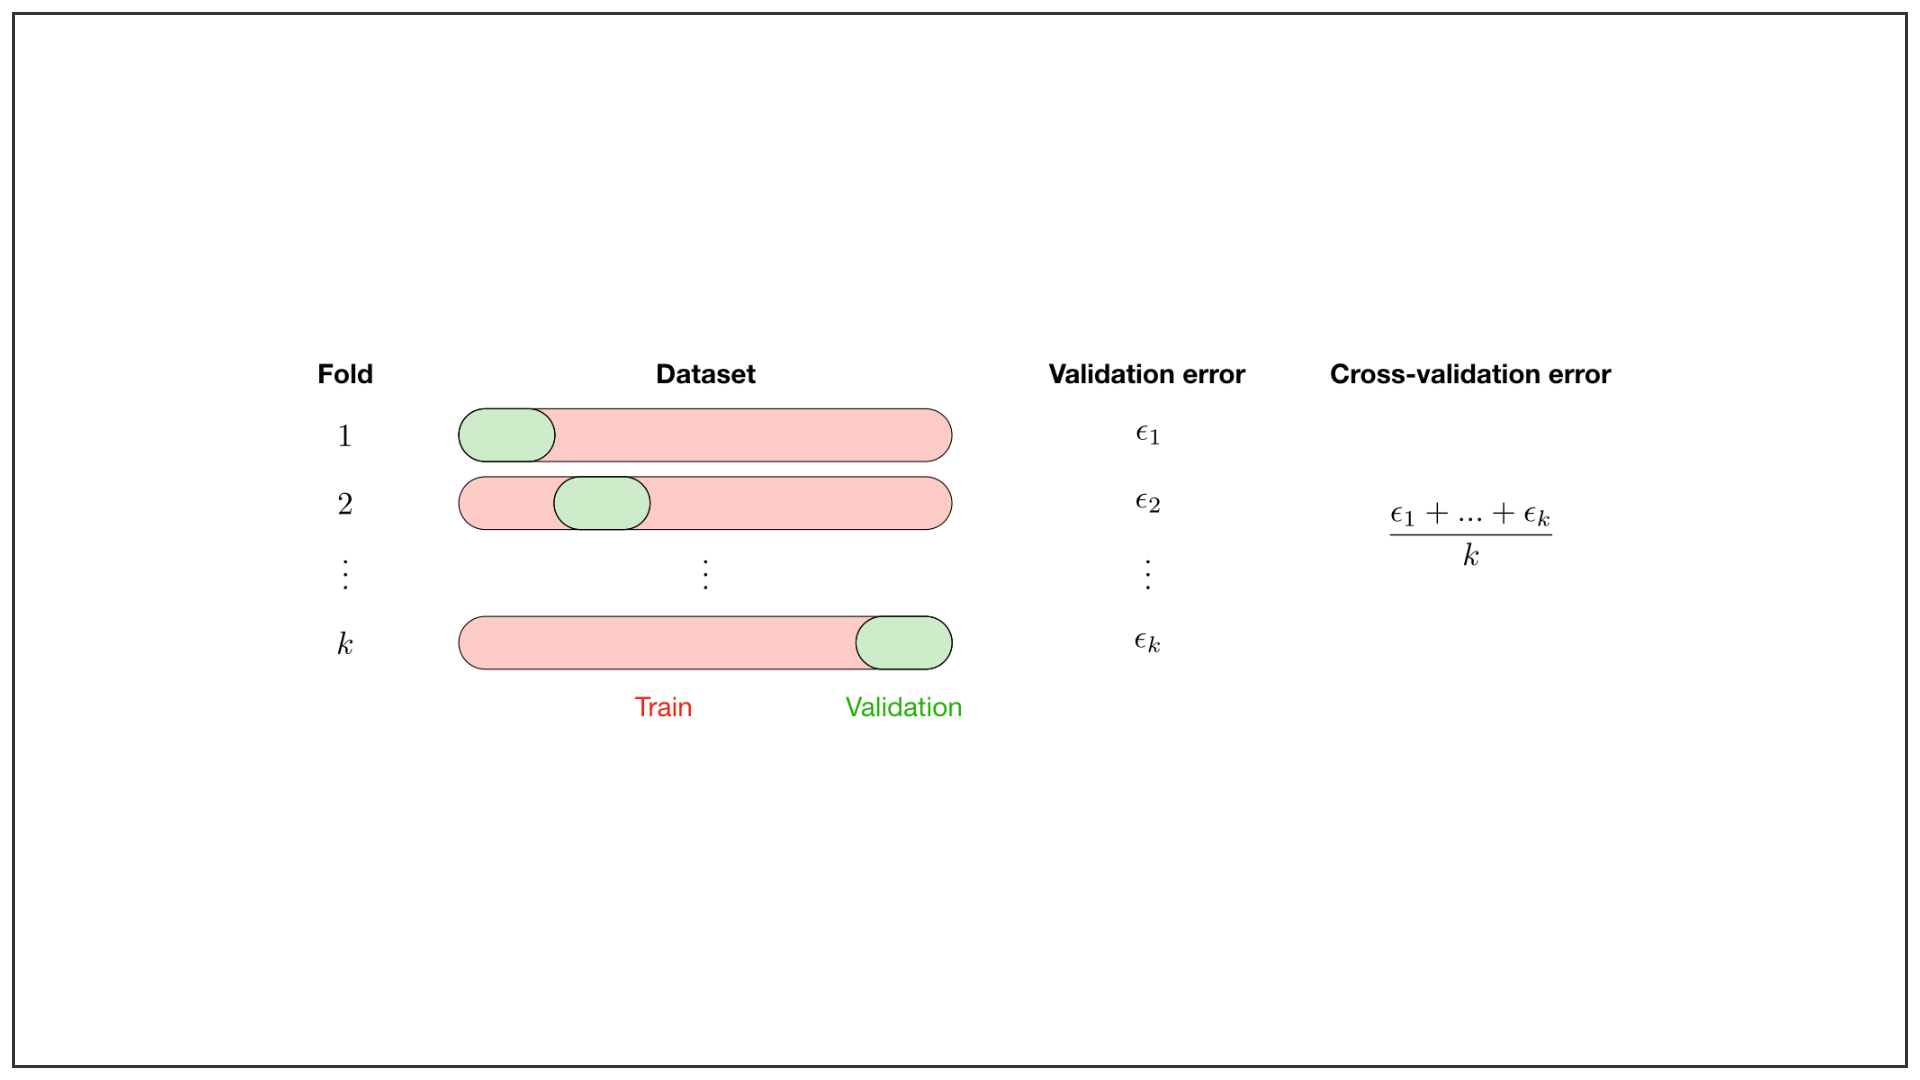
\includegraphics[width=\linewidth]{img//5/5.png}
    \caption{Esempio di k-fold cross-validation.}
    \label{fig:5-5}
\end{figure}

Prima di selezionare un modello per l'apprendimento, bisogna affrontare dinamiche fondamentali, come la capacità del modello di apprendere dai dati e la scelta degli iperparamentri. Per eseguire queste operazioni, viene suddiviso il dataset in diversi sottoinsiemi:

\begin{itemize}
    \item \textbf{Training set}: La parte di dataset destinata all'apprendimento.
    \item \textbf{Validation set}: È una porzione di dati utilizzata per valutare il modello.
    \item \textbf{Testing set}: Il sottoinsieme impiegato per le previsioni e i risultati.
\end{itemize}

\subsection{Cross-validation}

La cross-validation è una metodologia impiegata per scegliere un modello che non sia eccessivamente dipendente dal dataset di addestramento originale, ovvero dalla distribuzione dei dati del training set.

\bigskip

La figura \ref{fig:5-5}, illustra la k-fold cross-validation, una tra le possibili implementazioni di cross-validation, che è stata impiegata anche nel progetto connesso alla seguente tesi.

\paragraph{K-fold cross-validation}

\begin{enumerate}
    \item Il dataset viene suddiviso in k parti (fold) di uguali dimensioni. Per ogni fold, il modello viene addestrato sui dati di \( k-1 \) fold e validato sul fold rimanente.
    \item Questo processo è ripetuto k volte, con ogni fold utilizzato una volta come validation set.
    \item Per ogni fold, veongono registrati gli errori di validazione. L'errore di convalida è calcolato come la media degli errori di validazione dei singoli fold.
\end{enumerate}

\section{Metriche di performance}

\begin{figure}[t]
    \begin{multicols}{2}
        \centering
        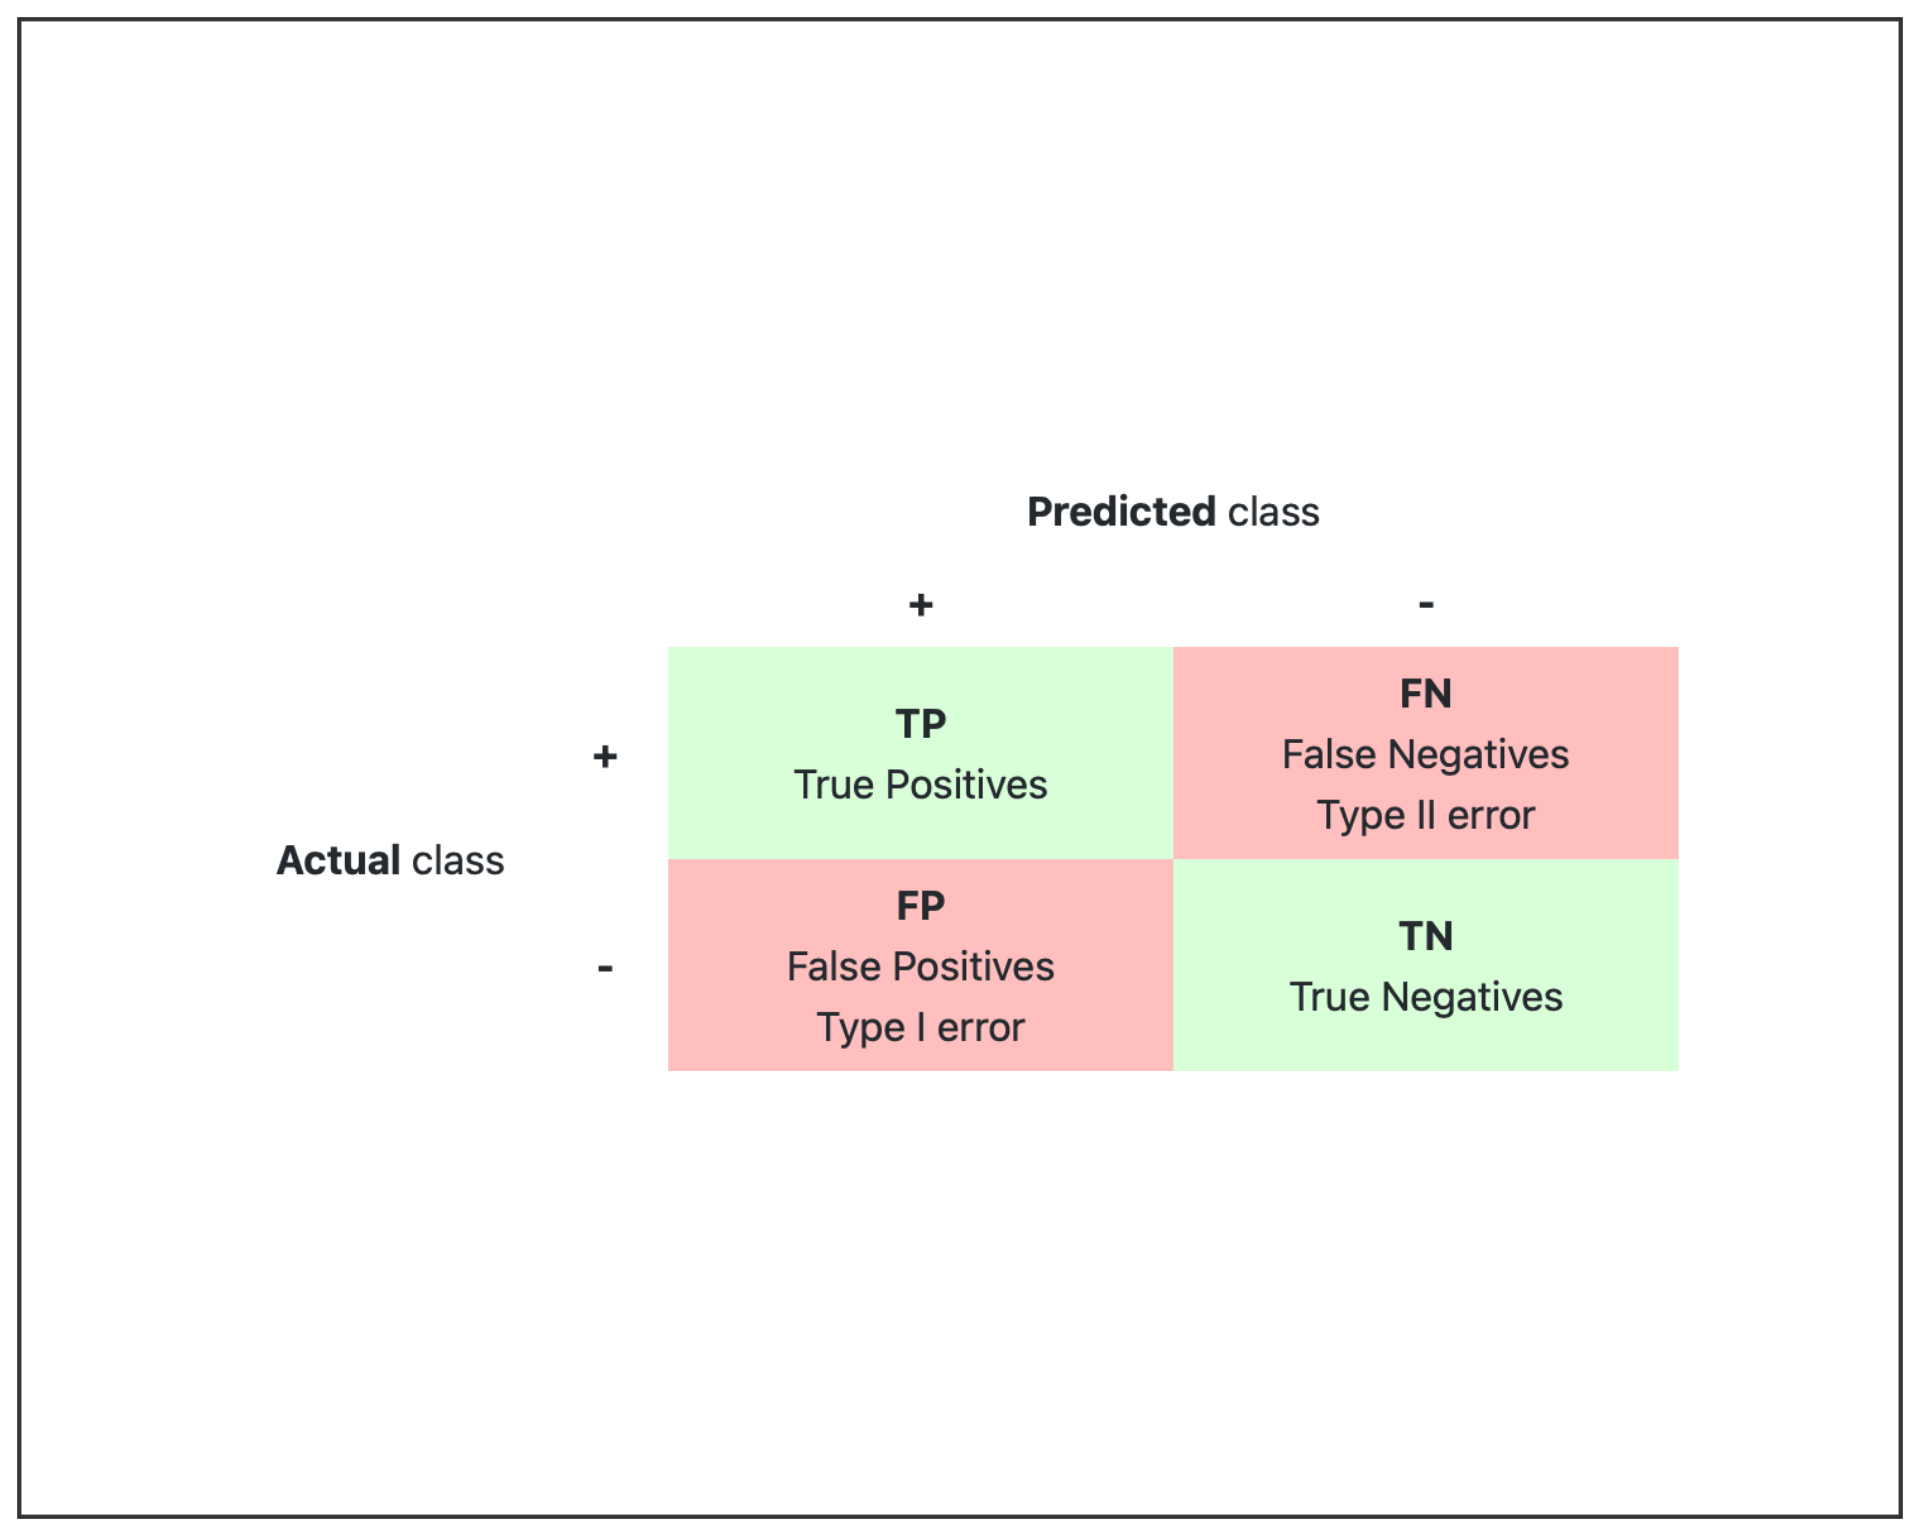
\includegraphics[width=\linewidth]{img//5/6.png}
        \caption{Matrice di confusione che illustra la classificazione binaria dei risultati di un modello predittivo.}
        \label{fig:5-6}
        
        \columnbreak
        
        \includegraphics[width=\linewidth]{img//5/7.png}
        \caption{Grafico silhouette di un clustering utilizzando il k-means.}
        \label{fig:5-7}
    \end{multicols}
\end{figure}

Per valutare in modo completo le prestazioni dei modelli, sono state impiegate diverse metriche. Queste metriche possono variare in base al tipo di modello selezionato.

\bigskip

I modelli utilizzati per la classificazione sono stati principalmente valutati utilizzando l'\textbf{accuratezza} come metrica di valutazione. L'accuratezza misura la proporzione di predizioni corrette rispetto al totale delle istanze nel dataset. L'equazione \ref{eq:5-4}, mostra la rappresentazione matematica dell'accuratezza.

\begin{equation}
    \boxed{
        \text{Accuracy} = \frac{TP + TN}{TP + TN + FP + FN}
    }
    \label{eq:5-4}
\end{equation}

\bigskip

Per ottenere una valutazione più completa delle prestazioni dei modelli di classificazione, è possibile utilizzare una \textbf{matrice di confusione}. La figura \ref{fig:5-6}, mostra la struttura di una matrice di confusione, nella quale sono riportati i risultati delle previsioni del modello rispetto alle classi effettive dei dati di test. Questa matrice è chiamata "di confusione" perché aiuta a comprendere quanto il modello possa confondersi tra le diverse classi.

\bigskip

I modelli che hanno utilizzato il clustering come tecnica di apprendimento, sono stati valutati utilizzando il \textbf{punteggio silhouette}. Questo punteggio, fornisce un'indicazione su quanto i punti dati all'interno di ogni cluster siano simili tra loro rispetto a quanto siano dissimili dai punti nei cluster adiacenti. Il punteggio silhouette varia da -1 a 1. Un punteggio positivo indica che l'oggetto è stato assegnato in modo appropriato al suo cluster, mentre un punteggio negativo indica che potrebbe essere assegnato a un cluster diverso. Un punteggio di zero suggerisce che l'oggetto è sulla soglia tra due cluster e potrebbe essere assegnato in modo ambiguo. Il calcolo di questo punteggio può essere effettuato mediante l'equazione \ref{eq:5-5}.

\begin{equation}
    \boxed{
        s = \frac{b - a}{\max(a, b)}
    }
    \label{eq:5-5}
\end{equation}

\bigskip

Dove \( a \) rappresenta la distanza media all'interno di un cluster e \( b \) rappresenta la distanza minima media tra un punto in un cluster e i punti nel cluster adiacente più vicino.

\bigskip

Per ulteriori analisi dei risultati del clustering, è stato impiegato il \textbf{grafico silhouette}. La rappresentazione di questo diagramma è visibile nella figura \ref{fig:5-7}, che aiuta a individuare la corretta definizione dei cluster e la collocazione del punteggio silhouette.
\pagebreak

\setcounter{chapter}{5}
\pagestyle{fancy}

\fancyhf{}

\fancyhead[C]{Risultati}
\fancyfoot[C]{\thepage}

\fancypagestyle{plain}{
    \fancyhf{}
    \fancyfoot[C]{\thepage}
}

\chapter{Risultati}

\large

I risultati analizzati in questo capitolo fungono da solida base concettuale per orientare e alimentare riflessioni strategiche nell'ambito di potenziali sviluppi e progetti futuri correlati.

\bigskip

La presentazione dei risultati segue l'impiego completo di tutte le features illustrate nel capitolo 2, mostrando un quadro esaustivo delle dinamiche e delle metriche prodotte. Da sottolineare che il dataset fornito includeva già le features calcolate, rimuovendo così il processo dalla necessità di convertire il segnale dell'elettrocardiogramma in valori numerici.

\section{Preprocessing dei dati}

\begin{table}[t]
    \centering
    \begin{tabular}{|lrrrrcr|}
        \hline
        & \textbf{MEAN\_RR}
        & \textbf{MEDIAN\_RR}
        & \textbf{SDRR}
        & \textbf{RMSSD}
        & ...
        & \textbf{condition} \\
        \hline        
        count
        & 369289
        & 369289
        & 369289
        & 369289
        & ...
        & 369289 \\
        unique
        & NaN
        & NaN
        & NaN
        & NaN
        & ...
        & 3 \\
        top
        & NaN
        & NaN
        & NaN
        & NaN
        & ...
        & no stress \\
        freq
        & NaN
        & NaN
        & NaN
        & NaN
        & ...
        & 200082 \\
        mean
        & 846
        & 841
        & 109
        & 14
        & ...
        & NaN \\
        std
        & 124
        & 132
        & 77
        & 4
        & ...
        & NaN \\        
        min
        & 547
        & 517
        & 27
        & 5
        & ...
        & NaN \\        
        25\%
        & 760
        & 755
        & 64
        & 11
        & ...
        & NaN \\
        50\%
        & 822
        & 819
        & 82
        & 14
        & ...
        & NaN \\
        75\%
        & 924
        & 916
        & 118
        & 17
        & ...
        & NaN \\
        max
        & 1322
        & 1653
        & 563
        & 26
        & ...
        & NaN \\
        \hline
    \end{tabular}
    \caption{Riepilogo delle statistiche del dataset prima del preprocessing.}
    \label{tab:6-1}
\end{table}

Per cominciare, è stata studiata la struttura del dataset al fine di identificare le strategie di preprocessing da impiegare. In particolare, si è concentrata l'attenzione sul training set poiché è la parte di dataset utilizzata dalla macchina per apprendere e successivamente predire il testing set. Dopo una prima esecuzione, è stata eseguita un'analisi preliminare che ha permesso di ottenere un insieme di statistiche per ciascuna delle feature presenti, le quali sono riportate nella tabella \ref{tab:6-1}.

\bigskip

Grazie a questo riepilogo, è stata progettata l'implementazione del preprocessing secondo le seguenti considerazioni:

\begin{itemize}
    \item In base al riepilogo, sembra che non ci siano valori mancanti nelle features numeriche, poiché il conteggio per ogni feature è coerente.
    \item La label \texttt{condition} è una variabile categorica e ha tre valori unici. Questa feature deve essere codificata in un formato numerico adatto alla modellazione.
    \item La variabile \texttt{datasetId} ha un valore costante per tutte le osservazioni. Questa feature può essere eliminata perché non fornisce alcuna variabilità o informazione utile per l'analisi o la modellazione predittiva.
    \item Le features hanno intervalli e scale diverse, come si deduce dai valori minimi, massimi e dalle deviazioni standard. Questa differenza di scala può causare problemi con alcuni tipi di modelli. Si può prendere in considerazione la standardizzazione.
    \item L'ampia quantità di features potrebbe complicare la previsione del modello. Le tecniche di riduzione della dimensionalità, come la PCA, sono utilizzate per semplificare il dataset, riducendo il numero di variabili, mentre si cerca di mantenere il massimo delle informazioni rilevanti.
\end{itemize}

\bigskip

\begin{figure}[t]
    \begin{multicols}{2}
        \centering
        \includegraphics[width=\linewidth]{img//6/1.png}
        \caption{Matrice di correlazione con le features del dataset prima del preprocessing dei dati.}
        \label{fig:6-1}
        
        \columnbreak
        
        \includegraphics[width=\linewidth]{img//6/2.png}
        \caption{Diagramma a torta che mostra la percentuale di individui che hanno sperimentato ciascuna delle condizioni di stress durante l'esperimento.}
        \label{fig:6-2}
    \end{multicols}
\end{figure}

La figura \ref{fig:6-1}, presenta una matrice di correlazione costruita utilizzando le features del dataset prima del processo di preprocessing dei dati. La correlazione rappresenta la forza della relazione tra due variabili: una correlazione positiva indica un'associazione diretta tra le variabili, mentre una correlazione negativa indica un'associazione inversa tra le variabili.

\bigskip

La figura \ref{fig:6-2}, presenta un diagramma a torta che visualizza la percentuale di individui che hanno provato ciascuna delle condizioni di stress in questione durante l'esperimento.

\section{Classificazione}

\begin{figure}[t]
    \begin{multicols}{3}
        \centering
        \includegraphics[width=\linewidth]{img//6/3.png}
        \caption{Matrice di confusione del logistic regression.}
        \label{fig:6-3}
        
        \columnbreak
        
        \includegraphics[width=\linewidth]{img//6/4.png}
        \caption{Matrice di confusione del decision tree.}
        \label{fig:6-4}

        \columnbreak
        
        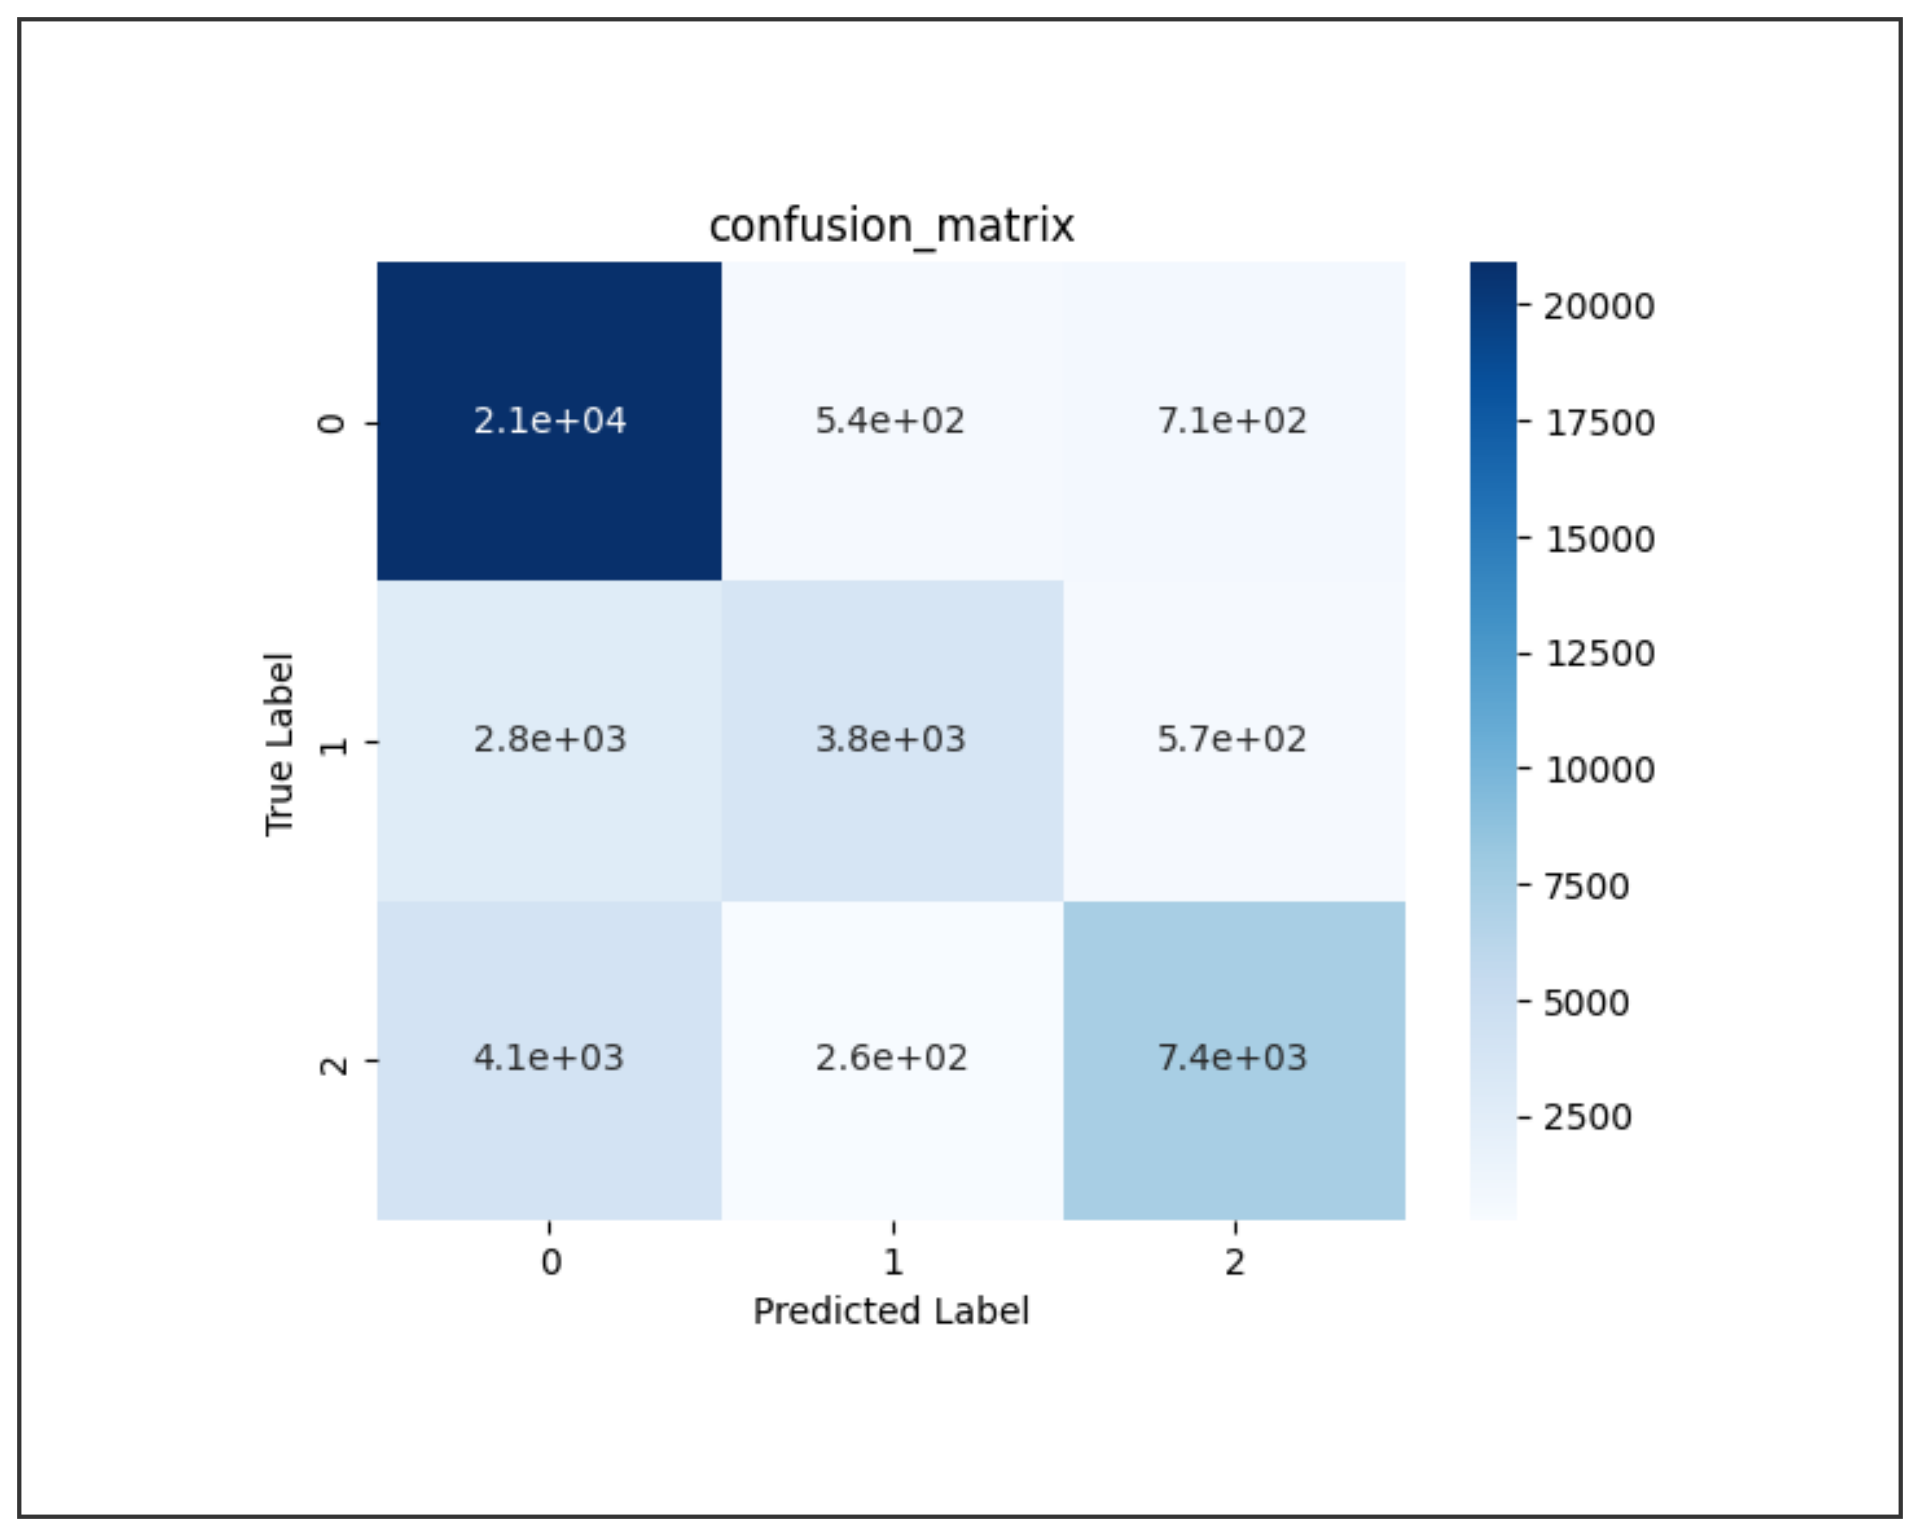
\includegraphics[width=\linewidth]{img//6/5.png}
        \caption{Matrice di confusione del random forest.}
        \label{fig:6-5}
    \end{multicols}
\end{figure}

Nel corso dell'apprendimento supervisionato, l'attenzione è stata concentrata esclusivamente sulla classificazione, con la valutazione di tre modelli: logistic regression, decision tree e random forest. L'obiettivo di questa scelta era esplorare le potenzialità e le prestazioni di ciascun modello, cercando di offrire una panoramica completa delle loro capacità e limitazioni nel problema correlato.

\subsection{Logistic regression}

\begin{table}[t]
    \centering
    \begin{tabular}{|r|rrrr|}
        \hline
        & \textbf{Precision}
        & \textbf{Recall}
        & \textbf{F1-score}
        & \textbf{Support} \\
        \hline
        \textbf{0}
        & 0.63
        & 0.87
        & 0.73
        & 22158 \\
        \textbf{1}
        & 0.60
        & 0.29
        & 0.39
        & 7093 \\
        \textbf{2}
        & 0.52
        & 0.30
        & 0.38
        & 11782 \\
        \textbf{Accuracy}
        &
        &
        & 0.61
        & 41033 \\
        \textbf{Macro Avg}
        & 0.58
        & 0.49
        & 0.50
        & 41033 \\
        \textbf{Weighted Avg}
        & 0.59
        & 0.61
        & 0.57
        & 41033 \\
        \hline
    \end{tabular}
    \caption{Risultati e metriche di performance del logistic regression.}
    \label{tab:6-2}
\end{table}

Come prima cosa, sono stati provati gli iperparametri adottati dagli autori del paper di riferimento \cite{iqbal2022exploring}. L'implementazione del modello è stata realizzata nel modo seguente:

\bigskip

\begin{lstlisting}
logistic_regression = LogisticRegression(
    solver='lbfgs',
    penalty='l2'
)
\end{lstlisting}

\bigskip

La tabella \ref{tab:6-2}, presenta i risultati e le metriche di performance ottenute a seguito di un'esecuzione del modello.

\bigskip

In conclusione, è stata realizzata una cross-validation su 10 fold, la media di questi valori, ha ottenuto un'accuratezza del 60.18\%.

\bigskip

Nella figura \ref{fig:6-3}, emerge dalla matrice di confusione che il modello mostra una buona capacità di predizione per la classe 0, con un numero significativo di predizioni corrette. Tuttavia, è evidente una certa confusione nella classe 1, dove il numero di falsi positivi è notevolmente superiore al numero di veri positivi. La classe 2 presenta una situazione simile, con un numero significativo di falsi positivi rispetto ai veri positivi.

\subsection{Decision tree}

\begin{table}[t]
    \centering
    \begin{tabular}{|r|rrrr|}
    \hline
    & \textbf{Precision}
    & \textbf{Recall}
    & \textbf{F1-Score}
    & \textbf{Support} \\
    \hline
    \textbf{0}
    & 0.64
    & 0.95
    & 0.76
    & 22158 \\
    \textbf{1}
    & 0.71
    & 0.37
    & 0.49
    & 7093 \\
    \textbf{2}
    & 0.80
    & 0.28
    & 0.42
    & 11782 \\
    \textbf{Accuracy}
    &
    &
    & 0.66
    & 41033 \\
    \textbf{Macro Avg}
    & 0.72
    & 0.53
    & 0.56
    & 41033 \\
    \textbf{Weighted Avg}
    & 0.70
    & 0.66
    & 0.62
    & 41033 \\
    \hline
    \end{tabular}
    \caption{Risultati e metriche di performance del decision tree.}
    \label{tab:6-3}
\end{table}

Inizialmente, sono stati ottimizzati gli iperparametri indicati dagli autori \cite{iqbal2022exploring}, poiché la vasta quantità di dati causava overfitting, portando il modello a una situazione di overtraining e generando prestazioni non realistiche. È stato necessario solo ridurre la profondità dell'apprendimento. L'implementazione pratica del modello è stata eseguita come segue:

\bigskip

\begin{lstlisting}
decision_tree = DecisionTreeClassifier(
    criterion='gini',
    max_depth=8,
    max_features='log2'
)
\end{lstlisting}

\bigskip

La tabella \ref{tab:6-3}, presenta i risultati e le metriche di performance generati in seguito all'esecuzione del modello.

\bigskip

In conclusione, è stata condotta una cross-validation su 10 fold, e la media di questi valori ha risultato in un'accuratezza del 74.47\%.

\bigskip

Nella figura \ref{fig:6-4}, si evidenzia dalla matrice di confusione che il modello mostra un'elevata precisione nella previsione della classe 0, con un numero significativo di predizioni corrette. Tuttavia, sono evidenti alcune aree di miglioramento, in particolare nelle classi 1 e 2. La classe 1 presenta un numero di falsi positivi otevolmente superiore al numero di veri positivi, indicando una certa confusione nella classificazione. Analogamente, nella classe 2, il numero di falsi positivi è sostanzialmente maggiore rispetto ai veri positivi.

\subsection{Random forest}

\begin{table}[t]
    \centering
    \begin{tabular}{|r|rrrr|}
        \hline
        & \textbf{Precision}
        & \textbf{Recall}
        & \textbf{F1-score}
        & \textbf{Support} \\
        \hline
        \textbf{0}
        & 0.74
        & 0.96
        & 0.83
        & 22158 \\
        \textbf{1}
        & 0.79
        & 0.51
        & 0.62
        & 7093 \\
        \textbf{2}
        & 0.89
        & 0.59
        & 0.71
        & 11782 \\
        \textbf{Accuracy}
        &
        &
        & 0.77
        & 41033 \\
        \textbf{Macro Avg}
        & 0.81
        & 0.68
        & 0.72
        & 41033 \\
        \textbf{Weighted Avg}
        & 0.79
        & 0.77
        & 0.76
        & 41033 \\
        \hline
    \end{tabular}
    \caption{Risultati e metriche di performance del random forest.}
    \label{tab:6-4}
\end{table}

Inizialmente, si è proceduto ottimizzando gli iperparametri raccomandati dagli autori \cite{iqbal2022exploring} al fine di affrontare il problema dell'overfitting, seguiti dalla stessa procedura adottata per il modello precedente. L'implementazione del modello è stata eseguita nel modo seguente:

\bigskip

\begin{lstlisting}
random_forest = RandomForestClassifier(
    criterion='gini',
    max_depth=8,
    max_features='log2',
    n_estimators=4
)
\end{lstlisting}

\bigskip

La tabella \ref{tab:6-4}, presenta i risultati e le metriche di performance ottenute dopo l'esecuzione del modello.

\bigskip

In conclusione, si è effettuata una cross-validation su 10 fold, e la media di tali valori ha prodotto un'accuratezza del 81.73\%.

\bigskip

Nella figura \ref{fig:6-5}, si deduce dalla matrice di confusione che il modello dimostra un'eccellente capacità di predizione nella classe 0, con un notevole numero di predizioni corrette. Tuttavia, sono presenti alcune aree di miglioramento nelle classi 1 e 2. Nella classe 1, il numero di falsi positivi supera considerevolmente il numero di veri positivi, indicando una certa confusione nella classificazione. Anche nella classe 2, il numero di falsi positivi è notevolmente superiore rispetto ai veri positivi.

\section{Clustering}

\begin{figure}[t]
    \begin{multicols}{3}
        \centering
        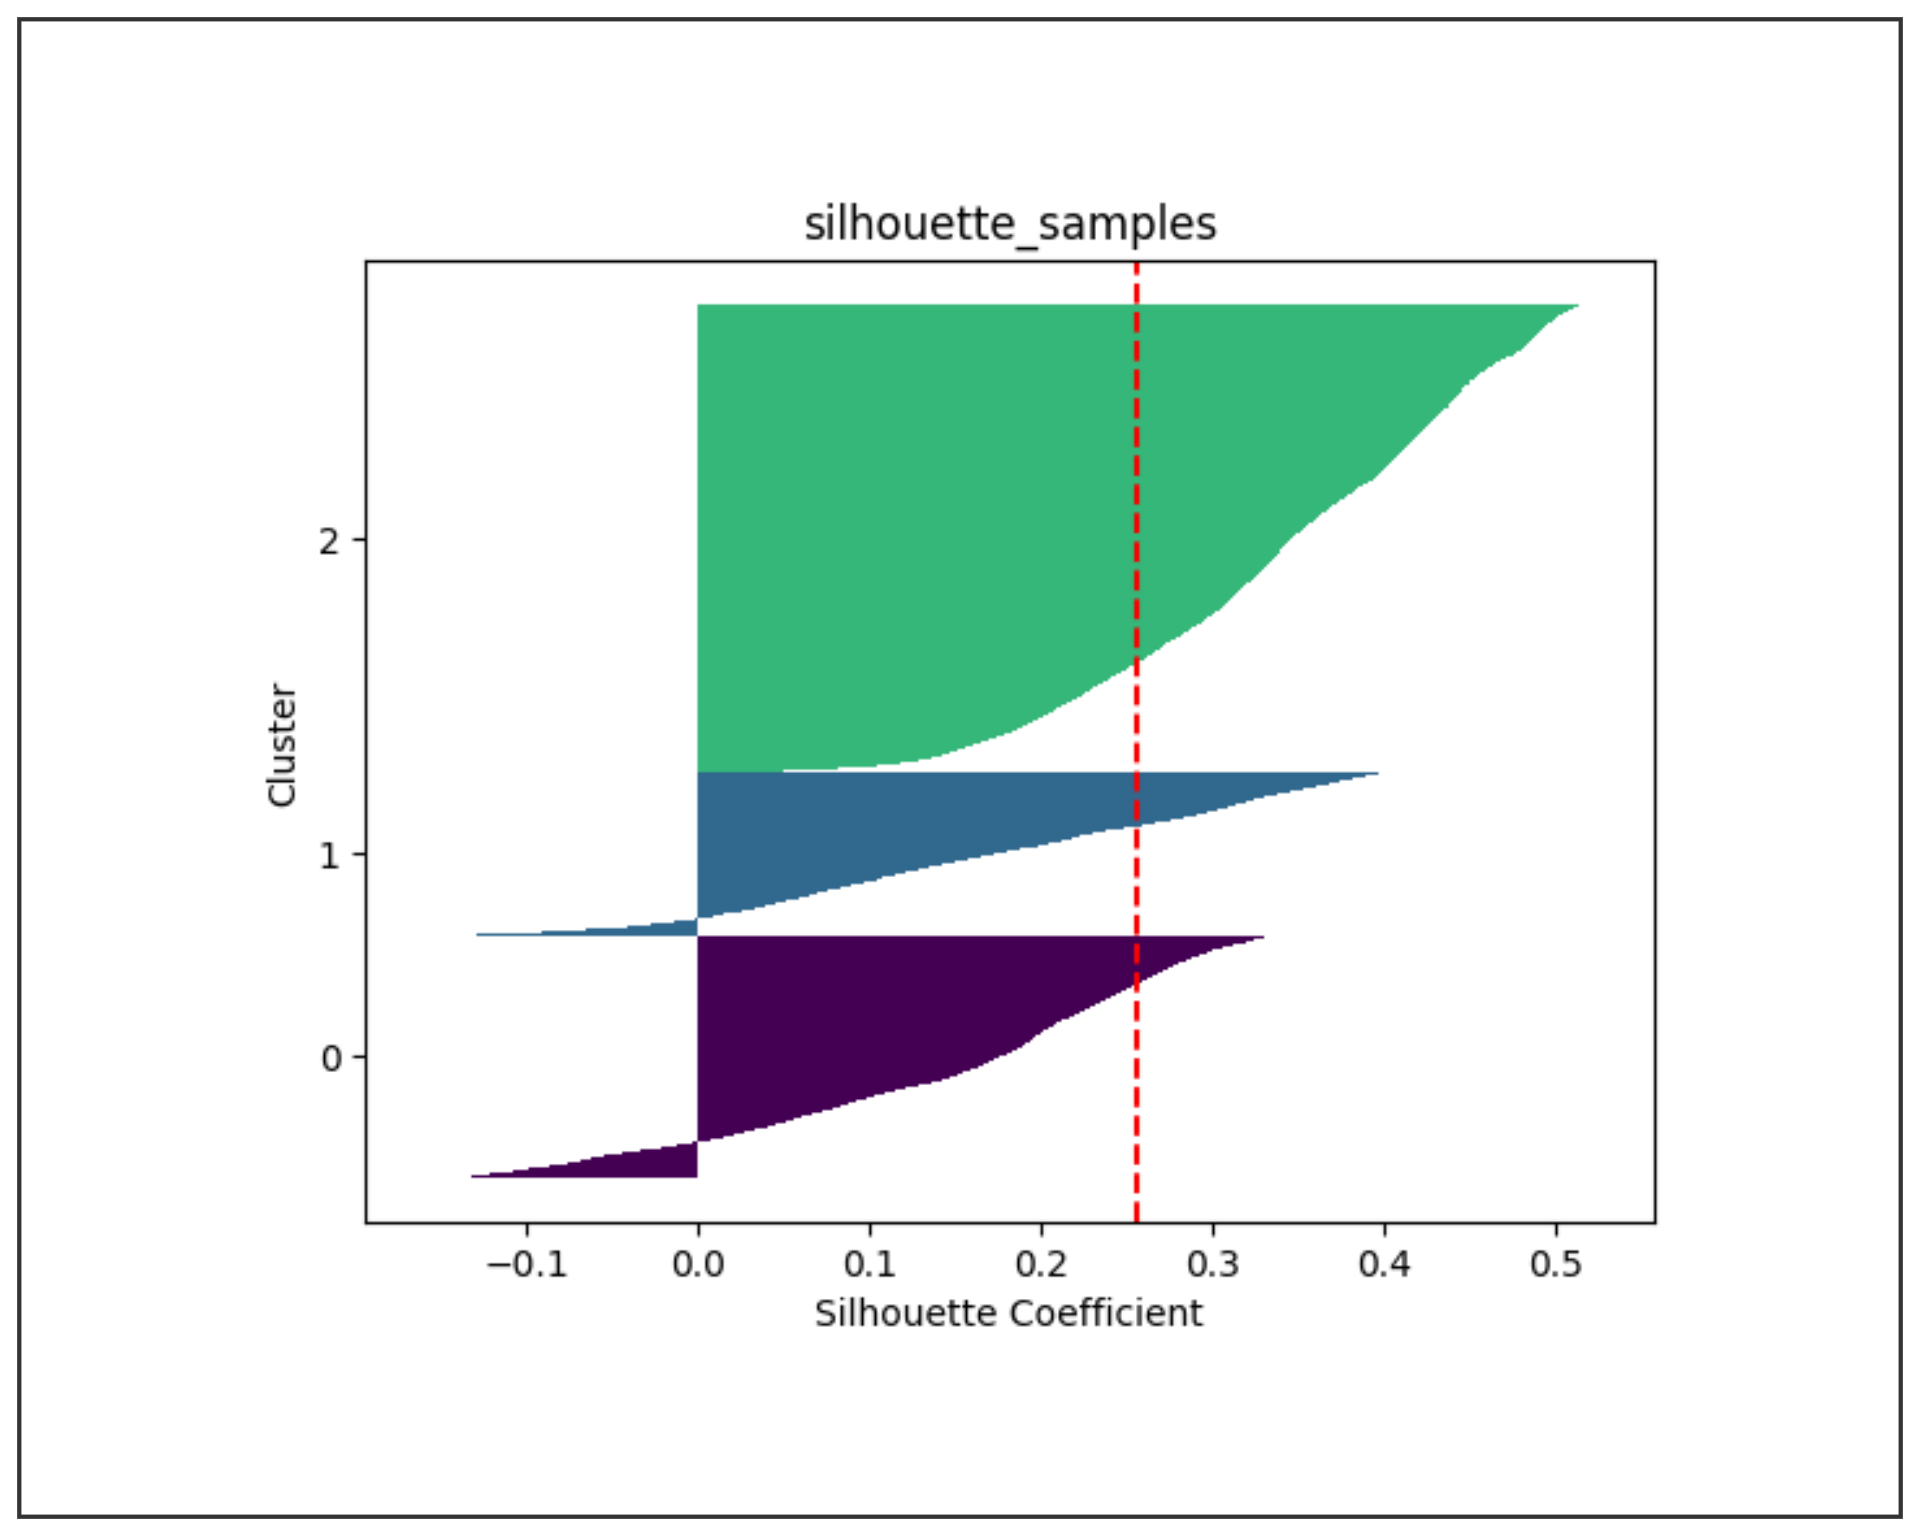
\includegraphics[width=\linewidth]{img//6/6.png}
        \caption{Grafico silhouette del k-means.}
        \label{fig:6-6}
        
        \columnbreak
        
        \includegraphics[width=\linewidth]{img//6/7.png}
        \caption{Grafico silhouette del gaussian mixture.}
        \label{fig:6-7}

        \columnbreak
        
        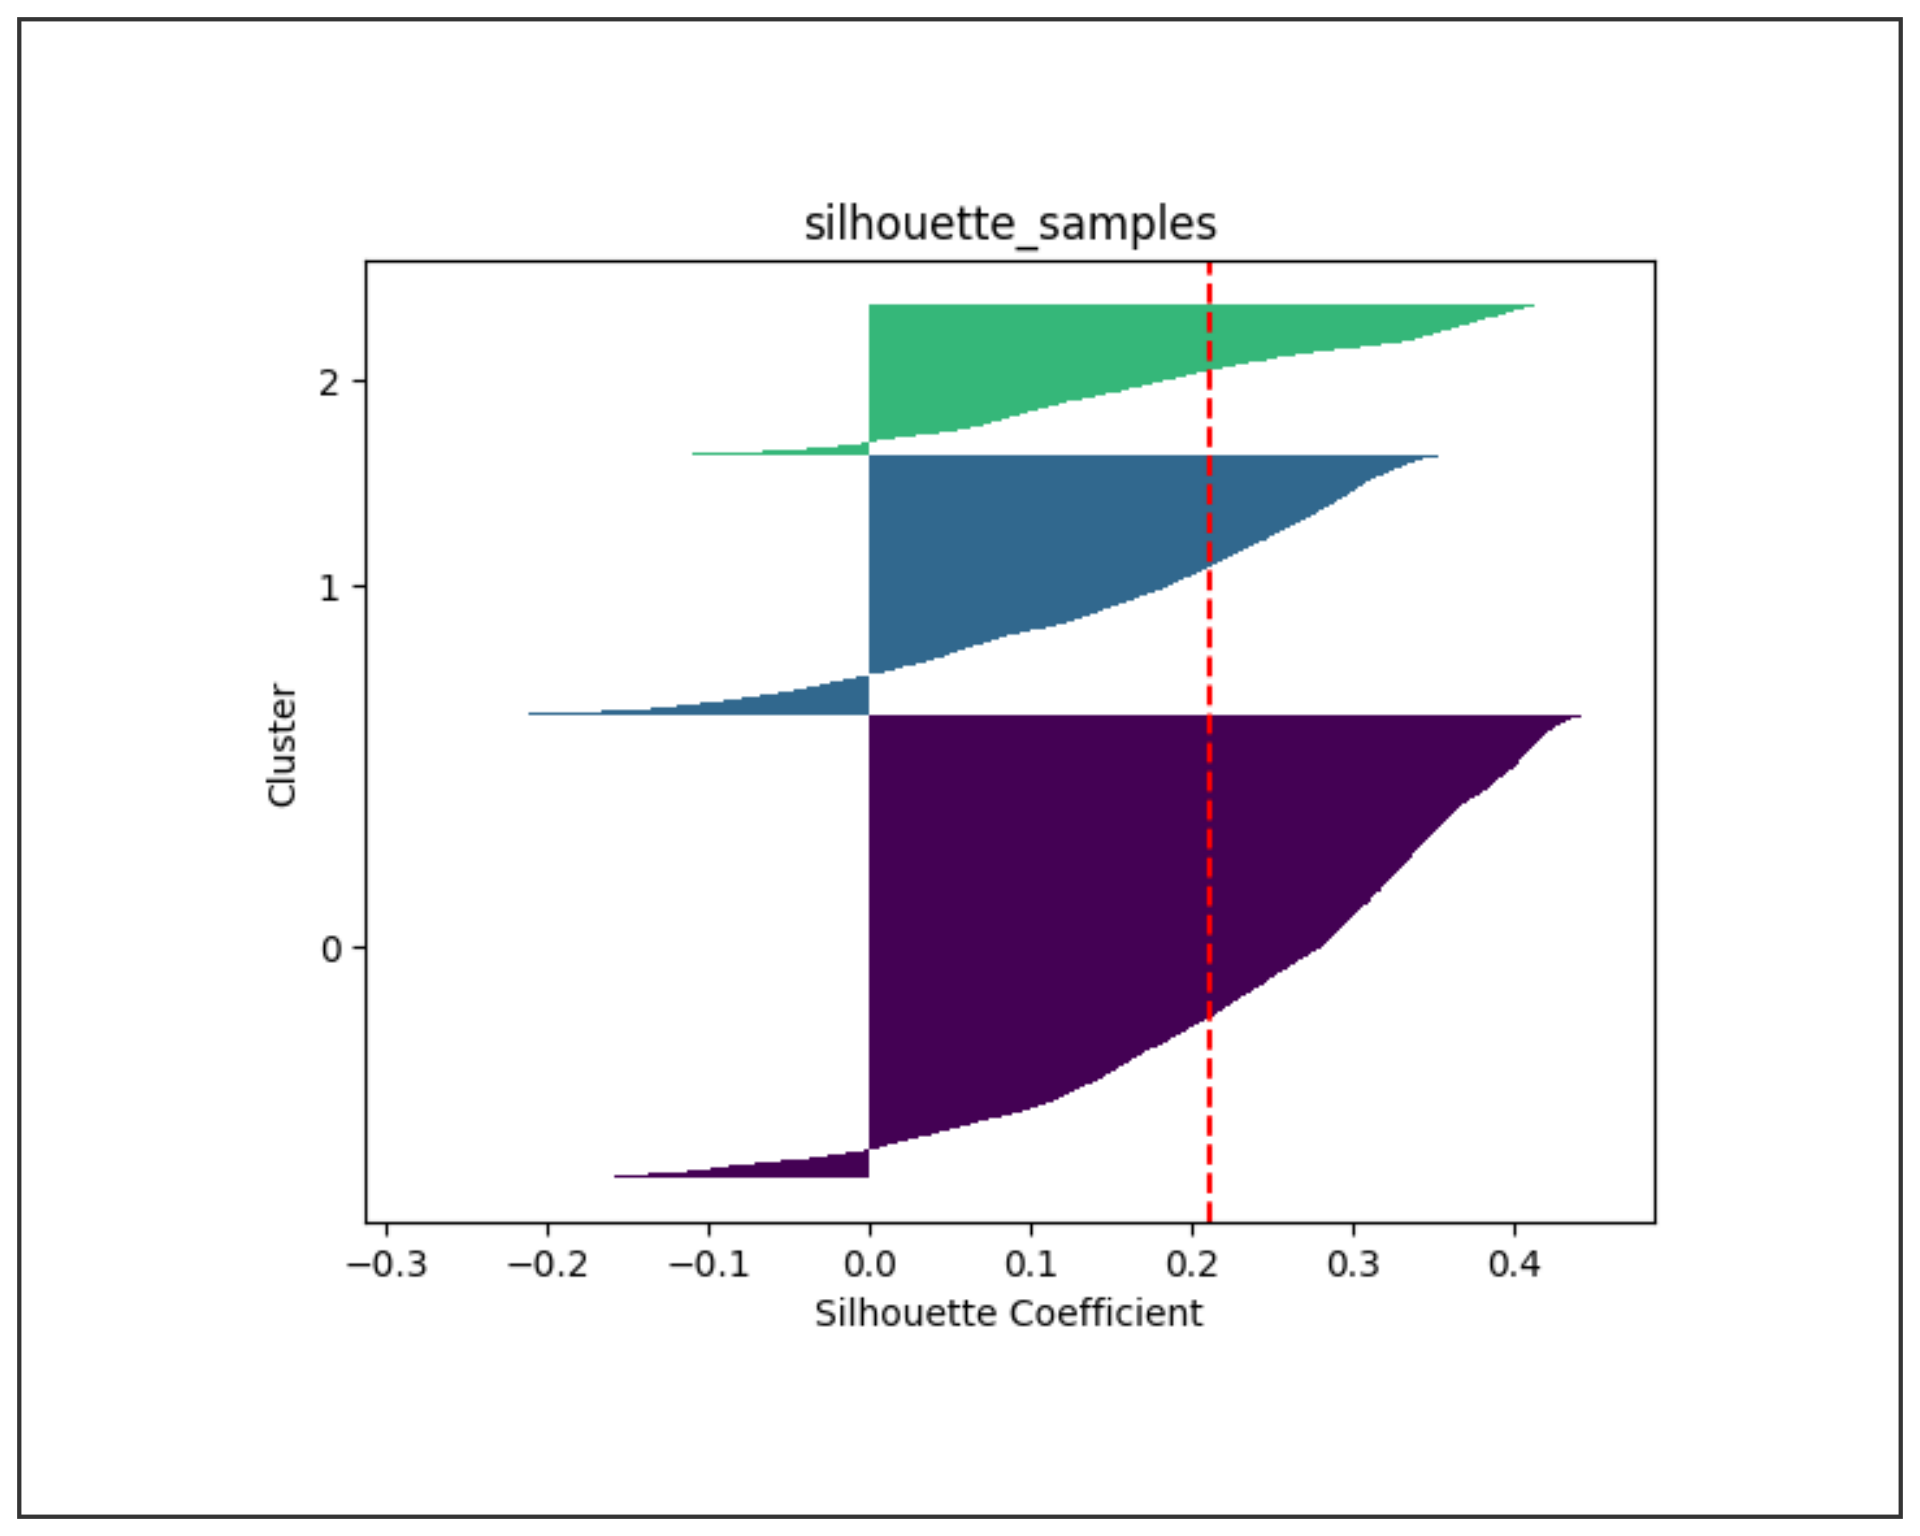
\includegraphics[width=\linewidth]{img//6/8.png}
        \caption{Grafico silhouette del BIRCH.}
        \label{fig:6-8}
    \end{multicols}
\end{figure}

Per l'apprendimento non supervisionato, il focus principale è stato sul clustering. Nello specifico, sono stati sperimentati tre modelli: k-means, gaussian mixture e BIRCH. Questa selezione è stata fatta per esplorare le potenzialità e le performance di ciascun modello, con lo scopo specifico di confrontare le prestazioni tra approcci supervisionati e non supervisionati.

\subsection{K-means}

Per cominciare, è stato fondamentale determinare il numero di cluster da utilizzare. Sebbene gli autori \cite{iqbal2022exploring} consigliassero l'impiego di due cluster, l'analisi ha dimostrato che con tre cluster le prestazioni miglioravano. Il modello è stato implementato nel modo seguente:

\bigskip

\begin{lstlisting}
kmeans = KMeans(n_clusters=3)
\end{lstlisting}

\bigskip

Il modello ha individuato un valore di punteggio silhouette pari a 0.2562, indicando così la coerenza e la distinzione efficace dei cluster nell'analisi.

\bigskip

Nella figura \ref{fig:6-6}, il coefficiente silhouette manifesta un valore medio di 0.2. Tale dato sottolinea la coerenza nelle definizioni e nelle distinzioni delle strutture dei dati oggetto dell'analisi.

\subsection{Gaussian mixture}

Inizialmente, è stato necessario determinare il numero di cluster; sebbene gli autori \cite{iqbal2022exploring} consigliassero l'uso di due cluster, l'adozione di tre ha portato a risultati migliori in termini di prestazioni. Di conseguenza, l'implementazione del modello è stata realizzata nel seguente modo:

\bigskip

\begin{lstlisting}
gaussian_mixture = GaussianMixture(n_components=3)
\end{lstlisting}

\bigskip

Il modello ha identificato un coefficiente di silhouette pari a 0.0928, evidenziando una moderata coerenza e distinzione tra i cluster nell'analisi effettuata. Questo valore suggerisce una separazione delle osservazioni, seppur con una certa sovrapposizione, indicando una struttura ragionevole ma potenzialmente migliorabile dei cluster identificati.

\bigskip

Nella figura \ref{fig:6-7}, il coefficiente silhouette manifesta un valore medio di 0.1. Tale dato sottolinea una misura di coerenza nelle definizioni delle strutture dei dati analizzati, anche se con una minore distinzione rispetto ad altre situazioni in cui il coefficiente silhouette potrebbe assumere valori più elevati.

\subsection{BIRCH}

Inizialmente, è stato necessario determinare il numero di cluster; sebbene gli autori \cite{iqbal2022exploring} consigliassero l'uso di due cluster, l'adozione di tre ha portato a risultati migliori in termini di prestazioni. Di conseguenza, l'implementazione del modello è stata realizzata nel seguente modo:

\bigskip

\begin{lstlisting}
birch = Birch(n_clusters=3)
\end{lstlisting}

\bigskip

Il modello ha rilevato un coefficiente di silhouette di 0.2117, suggerendo una coerenza significativa e una distinzione efficace dei cluster nell'ambito dell'analisi.

\bigskip

Nella figura \ref{fig:6-8}, il coefficiente silhouette rivela un valore medio di 0.2. Questo dato evidenzia la consistenza nelle definizioni e nelle distinzioni delle strutture dei dati sottoposti all'analisi.

\section{Risultati dei modelli}

\begin{table}[t]
    \centering
    \begin{tabular}{|llll|}
        \hline
        \textbf{Algoritmo}
        & \textbf{Modello}
        & \textbf{Metrica}
        & \textbf{Punteggio} \\
        \hline
        Supervised
        & Logistic regression
        & Accuracy
        & 60.18\% \\
        Supervised
        & Decision tree
        & Accuracy
        & 74.47\% \\
        Supervised
        & Random forest
        & Accuracy
        & 81.73\% \\
        Unsupervised
        & K-means
        & Silhouette
        & 0.2562 \\
        Unsupervised
        & Gaussian mixture
        & Silhouette
        & 0.0928 \\
        Unsupervised
        & BIRCH
        & Silhouette
        & 0.2117 \\
        \hline
    \end{tabular}
    \caption{Risultati e metriche di performance dei diversi modelli.}
    \label{tab:6-5}
\end{table}

Nella tabella \ref{tab:6-5}, vengono presentate le prestazioni dei vari modelli esaminati nel contesto dello studio. Tra i modelli di classificazione, il random forest mostra l'accuratezza più elevata, seguita dal decision tree e dal logistic regression. Per il clustering, i risultati indicano che sia il k-means che il BIRCH ottengono buone prestazioni, mentre il gaussian mixture mostra un punteggio silhouette molto più associato a zero.

\bigskip

In linea generale, i risultati evidenziano che per la classificazione sono efficaci sia il decision tree che il random forest, mentre per il clustering si distinguono per efficacia il k-means e il BIRCH. È interessante notare che le buone prestazioni sono comparabili tra i metodi supervisionati e quelli non supervisionati, suggerendo una parità di efficienza tra le due metodologie.

\bigskip

Attraverso il notebook disponibile su \href{https://www.kaggle.com/code/robertovicario/swell-kw-stress-detection}{\underline{Kaggle}}, è possibile esplorare in dettaglio tutti i risultati acquisiti, accompagnati dai codici associati. Questa piattaforma fornisce un'interfaccia diretta per visualizzare e analizzare in profondità i dati e le implementazioni sottostanti.
\pagebreak

\setcounter{chapter}{6}
\pagestyle{fancy}

\fancyhf{}

\fancyhead[C]{Conclusione}
\fancyfoot[C]{\thepage}

\fancypagestyle{plain}{
    \fancyhf{}
    \fancyfoot[C]{\thepage}
}

\chapter{Conclusione}

\large

La presente tesi ha esplorato l'efficacia di diversi metodi di machine learning per il rilevamento dello stress negli ambienti di lavoro d'ufficio. I risultati ottenuti hanno fornito importanti intuizioni su come lo stress impatti i dipendenti in diversi contesti lavorativi e hanno evidenziato l'efficacia di specifici strumenti di rilevamento.

\bigskip

Gli autori del dataset SWELL-KW, attraverso l'uso di questionari, monitoraggio fisiologico e interviste, hanno osservato che i livelli di stress possono variare notevolmente in base a fattori come il carico di lavoro, il clima organizzativo e le relazioni interpersonali sul posto di lavoro. Gli strumenti di rilevamento utilizzati si sono dimostrati validi per identificare i segnali di stress e per aiutare le organizzazioni a sviluppare interventi mirati.

\bigskip

In particolare, i test hanno confermato che l'apprendimento supervisionato è in grado di effettuare previsioni più precise. Allo stesso tempo, i modelli non supervisionati non mostrano prestazioni particolarmente scadenti, ma sembrano richiedere dati aggiuntivi per creare cluster più compatti. Questo risultato riafferma quanto evidenziato nel capitolo sullo stato dell'arte: i modelli di deep learning, come le reti neurali, e quelli basati su architetture con nodi e connessioni, si dimostrano estremamente efficaci.

\bigskip

Questo paragrafo, è dedicato a eventuali progetti futuri, in quanto questo progetto potrebbe essere approfondito. Pur essendo il dataset pubblicamente accessibile su Kaggle, è importante notare che i segnali provenienti dall'elettrocardiogramma sono già stati preprocessati e convertiti in dati numerici, così escludendo al pubblico una fase significativa di ricerca. Un secondo punto critico riguarda la grande quantità di dati presente nel dataset, che può portare alcuni modelli a soffrire di overtraining. Questo aspetto è rilevante poiché molti notebook online trascurano tale problematica, compromettendo la realistica interpretazione dei risultati dei loro studi. Infine, sarebbe interessante esplorare l'approccio del deep learning per valutare le prestazioni dei modelli e la loro capacità di apprendere e predire in modo accurato.

\bigskip

In conclusione, questo studio ha evidenziato l'importanza di un approccio basato sui dati per affrontare il problema dello stress negli ambienti di lavoro. Continuando a sviluppare e implementare strategie efficaci, è possibile creare ambienti lavorativi più sani e produttivi.
\newpage
\thispagestyle{empty}
\mbox{}
\pagebreak

\setcounter{page}{1}
\pagenumbering{Alph}

\pagestyle{fancy}

\fancyhf{}

\fancyhead[C]{Bibliografia}
\fancyfoot[C]{\thepage}

\fancypagestyle{plain}{
    \fancyhf{}
    \fancyfoot[C]{\thepage}
}

\large

\printbibliography
\newpage
\thispagestyle{empty}
\mbox{}
\pagebreak

\end{document}